% !TeX root = ../complete.tex
\chapter{انرژی و توان در مدارهای \lr{CMOS}}
\label{chap:power}

وقتی خروجی یک گیت \lr{CMOS} تغییر می‌کند، منبع تغذیه چه مقدار
انرژی تحویل می‌دهد؟ چرا دو مدار با کار منطقی یکسان می‌توانند توان
متفاوتی مصرف کنند؟ چه بخشی از مصرف با توقف تغییر وضعیت باقی می‌ماند؟
برای پاسخ، ابتدا انرژی یک گذار را از روی مسیر جریان و تغییر ولتاژ
حساب می‌کنیم. سپس از تعداد گذارهای هر گره به توان متوسط مدار می‌رسیم.
در تصمیم‌های طراحی، توان ناشی از فعالیت و توانی را که در حالت ساکن
مصرف می‌شود در کنار محدودیت زمانی در نظر می‌گیریم.

برای مرور، از \NotesTopic{sec:foundation-circuits}{ولتاژ، جریان و انرژی}
و \NotesTopic{tab:foundation-gates}{جدول صحت گیت‌های پایه} شروع کنید.
شکل موج و مدل بار در \NotesTopic{sec:delay-transient}{آغاز فصل تأخیر}
به تشخیص نقطه شروع و پایان گذار کمک می‌کنند. در خواندن نخست، برای هر
مثال مسیر جریان و شکل موج گره را مشخص کنید. بعد از تحلیل گذارها،
به مدار ساکن برگردید و ببینید کدام مسیرها هنوز جریان دارند. در پایان،
برای مقایسه دو طرح یک کار مشخص و یک محدودیت زمانی مشترک انتخاب کنید.

% !TeX root = ../complete.tex
\section{از توان لحظه‌ای تا انرژی یک گذار}
\label{sec:power-energy}

\subsection{توان لحظه‌ای، انرژی و توان متوسط}
\label{sec:power-average}

انرژی با ژول اندازه‌گیری می‌شود. توان، نرخ مبادله انرژی برحسب وات است.
برای نمونه، یک وات یعنی مبادله یک ژول در یک ثانیه. اگر جریان
\(i(t)\) از پایانه مثبت یک عنصر وارد شود و اختلاف پتانسیل دو پایانه
\(v(t)\) باشد، توان جذب‌شده عنصر در زمان \(t\) از حاصل‌ضرب این دو
به دست می‌آید \cite[بخش \secnum{۵.۱.۱}، صفحه ۱۸۲]{weste}.
\begin{equation}
  p(t)=v(t)i(t).
  \label{eq:power-instantaneous}
\end{equation}
در این قرارداد، \(p(t)>0\) یعنی عنصر انرژی می‌گیرد و \(p(t)<0\)
یعنی به مدار انرژی می‌دهد. در تحلیل تغذیه، \(I_{DD}(t)\) را در جهت
خروج از پایانه مثبت منبع تعریف می‌کنیم. بنابراین \(V_{DD}I_{DD}(t)\)
توان تحویلی منبع است. واحد حاصل‌ضرب ولت و آمپر همان وات است.

برای محاسبه انرژی، بازه بین \(t_0\) و \(t_1\) را به تکه‌های زمانی
کوتاه تقسیم کنید. در هر تکه با طول \(\Delta t\)، اگر توان تقریباً
ثابت باشد، انرژی آن تکه تقریباً \(p(t)\Delta t\) است. جمع این
انرژی‌ها در حد تکه‌های بسیار کوتاه همان انتگرال توان است. توان متوسط
توان ثابتی است که در همان مدت، همان انرژی را مبادله می‌کند.
با \(T=t_1-t_0>0\)، از رابطه‌های انتگرال و میانگین استفاده می‌کنیم
\cite[صفحه ۱۸۲]{weste}.
\begin{equation}
  E=\int_{t_0}^{t_1}p(t)\,\mathrm{d}t,
  \qquad
  P_{\mathrm{avg}}=\frac{E}{T}.
  \label{eq:power-interval}
\end{equation}
روی نمودار توان برحسب زمان، انتگرال برابر مساحت علامت‌دار بین منحنی
و محور زمان است. اگر توان در نیمه نخست یک بازه‌ی
\qty{4}{\nano\second} برابر \qty{3}{\milli\watt} و در نیمه دوم
صفر باشد، تنها نیمه نخست در انرژی سهم دارد. تبدیل پیشوندها در حاصل‌ضرب
انرژی به‌صورت زیر دیده می‌شود.
\[
  E=(\qty{3e-3}{\watt})(\qty{2e-9}{\second})
    =\qty{6e-12}{\joule}
    =\qty{6}{\pico\joule}.
\]
این انرژی بر کل زمان \qty{4}{\nano\second} تقسیم می‌شود و توان
متوسط \qty{1.5}{\milli\watt} به دست می‌آید. اگر زمان انتظار بدون
مصرف طولانی‌تر شود، انرژی همان رویداد ثابت می‌ماند و توان متوسط در
بازه‌ی طولانی‌تر کم‌تر می‌شود.

\subsection{انرژی خازن و انرژی تحویلی منبع}
\label{sec:power-capacitor-energy}

یک \lr{Inverter} خروجی ورودی خود را معکوس می‌کند. وقتی ورودی از
یک به صفر می‌رود، \lr{pMOS} خروجی را به تغذیه وصل می‌کند. وقتی
ورودی از صفر به یک می‌رود، \lr{nMOS} خروجی را به زمین وصل می‌کند.
در مدل شکل \ref{fig:power-charge-paths}، بار خروجی خازن ثابت \(C_L\)
است. فرض می‌کنیم در هر گذار فقط مسیر نشان‌داده‌شده هدایت می‌کند،
منبع در \(V_{DD}\) ثابت می‌ماند و خروجی پیش از گذار بعدی به سطح
نهایی خود می‌رسد. این مدل با تقریب بارِ
\NotesTopic{sec:delay-inverter-transient}{پاسخ گذرای \lr{Inverter}}
سازگار است \cite[شکل \secnum{۵.۴}، صفحه ۱۸۳]{weste}.

\begin{figure}[htbp]
  \centering
  \begin{latin}
  \begin{tikzpicture}[x=1cm,y=1cm]
    \foreach \xx/\stage in {0/\(p\mathrm{MOS}\),6/\(n\mathrm{MOS}\)} {
      \begin{scope}[xshift=\xx cm]
        \draw[thick] (0,1.1) -- (0,0) -- (3,0) -- (3,0.46);
        \draw[thick] (2.73,0.46) -- (3.27,0.46);
        \draw[thick] (2.73,0.64) -- (3.27,0.64);
        \draw[thick] (3,0.64) -- (3,1.65) -- (1.55,1.65);
        \draw[thick] (1.55,1.4) rectangle (0.45,1.9);
        \node at (1,1.65) {\stage};
        \draw[thick] (0.45,1.65) -- (0,1.65) -- (0,1.1);
        \draw[thick] (2.72,0) -- (3.28,0);
        \draw[thick] (2.81,-0.12) -- (3.19,-0.12);
        \draw[thick] (2.91,-0.24) -- (3.09,-0.24);
        \fill (3,1.65) circle (1.5pt);
        \node[above] at (3,1.65) {\(v_o\)};
        \node[right] at (3.32,0.55) {\(C_L\)};
      \end{scope}
    }
    \draw[thick,fill=white] (0,0.75) circle (0.35);
    \node at (0,0.87) {\scriptsize \(+\)};
    \node at (0,0.63) {\scriptsize \(-\)};
    \node[left] at (-0.4,0.75) {\(V_{DD}\)};
    \draw[->,blue!70!black,thick] (1.65,1.39) -- (2.65,1.39)
      node[midway,below] {\(i_C\)};
    \draw[->,blue!70!black,thick] (8.65,1.39) -- (7.65,1.39)
      node[midway,below] {\(-i_C\)};
    \node[above] at (1.5,2.05) {\rl{شارژ}};
    \node[above] at (7.5,2.05) {\rl{تخلیه}};
  \end{tikzpicture}
  \end{latin}
  \caption{مسیر معادل شارژ و تخلیه بار خروجی یک \lr{Inverter}.
    \(i_C\) در جهت ورود به صفحه بالایی \(C_L\) تعریف شده است.
    در تخلیه، جهت جریان معکوس و بزرگی آن برابر \(-i_C\) است.
    مدار از تحلیل شکل \secnum{۵.۴} کتاب اقتباس شده است \cite{weste}.}
  \label{fig:power-charge-paths}
\end{figure}

طبق \NotesTopic{sec:foundation-capacitor}{مدل خازن ثابت}، بار صفحه
بالایی خازن در ولتاژ \(v_o\) برابر \(q=C_Lv_o\) است و جریان
\(i_C=\mathrm{d}q/\mathrm{d}t\) نرخ تغییر این بار را نشان می‌دهد.
وقتی بسته‌ی کوچک بار \(\mathrm{d}q\) وارد خازن می‌شود، از رابطه
\eqref{eq:power-instantaneous} انرژی جذب‌شده برابر
\(v_o\,\mathrm{d}q\) است. ولتاژ در طول شارژ تغییر می‌کند. بنابراین
برای محاسبه انرژی باید سهم هر بسته بار را با ولتاژ همان لحظه جمع کنیم.
با جای‌گذاری \(\mathrm{d}q=C_L\,\mathrm{d}v_o\)، انرژی ذخیره‌شده
پس از شارژ از صفر تا \(V_{DD}\) چنین است
\cite[رابطه‌های \secnum{۵.۶} و \secnum{۵.۷}، صفحات ۱۸۲ و ۱۸۳]{weste}.
\begin{equation}
  E_C=\int_{0}^{V_{DD}} C_Lv_o\,\mathrm{d}v_o
     =C_L\left[\frac{v_o^2}{2}\right]_{0}^{V_{DD}}
     =\frac{1}{2}C_LV_{DD}^2.
  \label{eq:power-capacitor-energy}
\end{equation}
مشتق \(v_o^2/2\) نسبت به \(v_o\) برابر \(v_o\) است. به همین دلیل
انتگرال با تفریق مقدار \(v_o^2/2\) در دو کران به دست می‌آید. روی نمودار
\(v_o\) برحسب \(q\) نیز همین انرژی مساحت مثلثی به قاعده
\(C_LV_{DD}\) و ارتفاع \(V_{DD}\) است.

در مسیر شارژ، تمام بارِ واردشده به خازن از پایانه مثبت منبع عبور
می‌کند. منبع برای هر واحد بار، انرژی متناظر با ولتاژ ثابت \(V_{DD}\)
را می‌دهد. پس برای یافتن انرژی تحویلی منبع \(E_{DD}\)، بار کل
\(Q=C_LV_{DD}\) را در \(V_{DD}\) ضرب می‌کنیم
\cite[رابطه \secnum{۵.۸}، صفحه ۱۸۳]{weste}
\cite[اسلایدهای ۳ تا ۵]{powerslides}.
\begin{equation}
  E_{DD}=\int_0^Q V_{DD}\,\mathrm{d}q
        =V_{DD}Q=C_LV_{DD}^2.
  \label{eq:power-source-energy}
\end{equation}
واحد \(C_LV_{DD}^2\) برابر فاراد ضرب‌در مربع ولت است. از آنجا که
فاراد برابر کولن بر ولت و ژول برابر ولت ضرب‌در کولن است، حاصل ژول
می‌شود. اختلاف \(E_{DD}-E_C\) در \lr{pMOS} به گرما تبدیل می‌شود.
در تخلیه، تغذیه از مسیر بار جداست و انرژی ذخیره‌شده در \lr{nMOS}
تلف می‌شود. در پایان چرخه، انرژی خازن به مقدار اولیه بازمی‌گردد و
مجموع انرژی تلف‌شده در دو مسیر برابر \(C_LV_{DD}^2\) است.

\subsection{مثال و کنترل موازنه انرژی}
\label{sec:power-cycle-example}

بار \qty{150}{\femto\farad} را با تغذیه \qty{1.0}{\volt} در
نظر بگیرید. این داده‌ها از مثال شکل موج اسلاید ۶ و شکل
\secnum{۵.۵} کتاب گرفته شده‌اند. محاسبه را با فرض‌های مدل شکل
\ref{fig:power-charge-paths} انجام می‌دهیم
\cite[اسلاید ۶]{powerslides}\cite[صفحات ۱۸۳ و ۱۸۴]{weste}.
\[
  E_{DD}=(\qty{150e-15}{\farad})(\qty{1.0}{\volt})^2
        =\qty{150}{\femto\joule},
  \qquad
  E_C=\frac{E_{DD}}{2}=\qty{75}{\femto\joule}.
\]
در شارژ، \qty{75}{\femto\joule} در \lr{pMOS} تلف و
\qty{75}{\femto\joule} در خازن ذخیره می‌شود. در تخلیه، همین انرژی
ذخیره‌شده در \lr{nMOS} به گرما تبدیل می‌شود. با ثابت بودن ظرفیت و
ولتاژ و کامل بودن شارژ و تخلیه، کندتر شدن گذار مقدار بار جابه‌جاشده و
انرژی این مدل را تغییر نمی‌دهد. شکل لحظه‌ای جریان و مدت گذار می‌توانند
تغییر کنند. بخش \ref{sec:power-short-circuit} سهم جریان مستقیم از
تغذیه به زمین را بررسی می‌کند.

% !TeX root = ../complete.tex
\section{برآورد \lr{Dynamic Power}}
\label{sec:power-dynamic}

\subsection{از شمارش گذار تا توان سوئیچینگ}
\label{sec:power-switching}

در یک بازه‌ی مشاهده به طول \(T\)، تعداد شارژهای کامل یک گره از صفر
تا \(V_{DD}\) را \(N_{\uparrow}\) می‌نامیم. با فرض‌های بخش
\ref{sec:power-capacitor-energy}، هر شارژ انرژی \(C_LV_{DD}^2\) را
از منبع می‌گیرد. \(f_{\mathrm{sw}}=N_{\uparrow}/T\) نرخ شارژها
برحسب تعداد در ثانیه است. بنابراین توان متوسطی که منبع برای شارژ بار
تحویل می‌دهد از رابطه زیر به دست می‌آید
\cite[رابطه‌های \secnum{۵.۹} و \secnum{۵.۱۰}، صفحه ۱۸۴]{weste}
\cite[اسلایدهای ۷ و ۸]{powerslides}.
\begin{equation}
  P_{\mathrm{sw}}=\frac{N_{\uparrow}C_LV_{DD}^2}{T}
                =C_LV_{DD}^2 f_{\mathrm{sw}}.
  \label{eq:power-switching-rate}
\end{equation}
برابری انرژی گرفته‌شده از منبع و انرژی تلف‌شده برای یک چرخه‌ی کامل
برقرار است. در بازه‌ای که ولتاژ ابتدا و انتهای آن متفاوت باشد، برای
حساب انرژی تلف‌شده باید تغییر انرژی ذخیره‌شده در خازن را هم لحاظ کرد.

\lr{Clock} سیگنالی دوره‌ای است که زمان عمل مدار را تعیین می‌کند.
اگر فرکانس ساعت \(f\) باشد، در بازه‌ای به طول \(T\) که دقیقاً شامل
تعدادی دوره کامل است، \(N_{\mathrm{clk}}=fT\) دوره داریم. با تقسیم
تعداد شارژها بر تعداد دوره‌ها، \lr{Activity Factor} را تعریف می‌کنیم.
\begin{equation}
  \alpha=\frac{N_{\uparrow}}{N_{\mathrm{clk}}}
        =\frac{f_{\mathrm{sw}}}{f}.
  \label{eq:power-activity-count}
\end{equation}
صورت و مخرجِ کسر اول شمارش‌اند. پس \(\alpha\) بی‌بعد است و میانگین
تعداد گذار صعودی در هر دوره ساعت را نشان می‌دهد. با جای‌گذاری
\(f_{\mathrm{sw}}=\alpha f\) در رابطه \eqref{eq:power-switching-rate}،
برآورد توان سوئیچینگ برحسب فرکانس ساعت چنین می‌شود.
\begin{equation}
  P_{\mathrm{sw}}=\alpha C_LV_{DD}^2 f.
  \label{eq:power-switching}
\end{equation}
در این قرارداد، تنها گذار \(0\to 1\) شمرده می‌شود. خود ساعت در هر
دوره یک لبه صعودی و یک لبه نزولی دارد، پس \(\alpha=1\) است. برای
داده‌ای که در هر دوره یک بار مقدارش عوض می‌شود، گذارها یکی‌درمیان
صعودی و نزولی‌اند. در یک بازه شامل تعداد زوج از این گذارها،
\(\alpha=1/2\) است. گره ثابت \(\alpha=0\) دارد. اگر خود گره بار
اسلاید ۶ در هر دوره ساعت \qty{1}{\giga\hertz} یک بار شارژ شود،
از انرژی بخش \ref{sec:power-cycle-example} به توان زیر می‌رسیم.
\[
  P_{\mathrm{sw}}=(\qty{150e-15}{\joule})(\qty{1e9}{\hertz})
                =\qty{150}{\micro\watt}.
\]
هرتز معادل معکوس ثانیه است. اگر همین گره به‌طور متوسط در هر دو دوره
یک بار شارژ شود، با همان انرژی به‌ازای هر شارژ، توان سوئیچینگ نصف
می‌شود.

\subsection{جمع سهم گره‌ها و تخمین توان یک تراشه}
\label{sec:power-effective-capacitance}

در یک شبکه چندگرهی، هر گره شماره \(i\) بار معادل \(C_i\) و
\lr{Activity Factor} مختص خود \(\alpha_i\) را دارد. بار شامل
ظرفیت ورودی گیت‌های متصل به گره، ظرفیت‌های \lr{Diffusion} روی گره
و ظرفیت سیم است. در مدل ساده، ولتاژ تغذیه و فرکانس را برای همه‌ی گره‌ها
مشترک می‌گیریم و \(\alpha_i C_i\) را ظرفیت مؤثرِ فعالیت آن گره
می‌نامیم. برای محاسبه توان، سهم گره‌ها را جمع می‌کنیم
\cite[بخش \secnum{۵.۲}، صفحه ۱۸۵]{weste}.
\begin{equation}
  P_{\mathrm{sw}}=V_{DD}^2 f\sum_i\alpha_i C_i.
  \label{eq:power-node-sum}
\end{equation}
برای گره‌هایی که تغذیه یا فرکانس متفاوت دارند، توان هر گروه را با
مقادیر همان گروه حساب می‌کنیم و سپس توان‌ها را با هم جمع می‌کنیم.

در مثال ۵.۱ کتاب و اسلایدهای ۱۱ و ۱۲، مدار به دو گروه منطق و حافظه
تقسیم شده است. در هر گروه، به‌جای محاسبه تک‌تک گره‌ها، از عرض متوسط
ترانزیستورها و یک \lr{Activity Factor} نماینده استفاده می‌کنیم. تعداد
ترانزیستورهای منطق \(50\times10^6\) و تعداد ترانزیستورهای حافظه
\(950\times10^6\) است. اگر واحد هندسی \(\lambda\) برابر
\qty{25}{\nano\metre} باشد، عرض‌های متوسط \(12\lambda\) و
\(4\lambda\) را از راه تبدیل واحد به‌ترتیب
\qty{0.30}{\micro\metre} و \qty{0.10}{\micro\metre} به دست
می‌آوریم. فرض مثال برای مجموع ظرفیت \lr{Gate} و \lr{Diffusion}،
\qty{1.8}{\femto\farad\per\micro\metre} به‌ازای هر واحد عرض است.
ظرفیت سیم و توان جریان مستقیم در این تخمین کنار گذاشته می‌شوند
\cite[مثال ۵.۱، صفحات ۱۸۵ و ۱۸۶]{weste}
\cite[اسلایدهای ۱۱ و ۱۲]{powerslides}.

با ضرب تعداد ترانزیستور در عرض متوسط و ظرفیت بر واحد عرض، ظرفیت
تجمیعی هر گروه به دست می‌آید. واحد طول در ضرب حذف می‌شود و حاصل
برحسب فاراد است.
\[
  \begin{aligned}
    C_{\mathrm{logic}}&=(50\times10^6)(\qty{0.30}{\micro\metre})
      (\qty[per-mode=symbol]{1.8}{\femto\farad\per\micro\metre})
      =\qty{27}{\nano\farad},\\
    C_{\mathrm{mem}}&=(950\times10^6)(\qty{0.10}{\micro\metre})
      (\qty[per-mode=symbol]{1.8}{\femto\farad\per\micro\metre})
      =\qty{171}{\nano\farad}.
  \end{aligned}
\]
با فعالیت \(0.1\) برای منطق و \(0.02\) برای حافظه، ظرفیت‌های مؤثر
\qty{2.7}{\nano\farad} و \qty{3.42}{\nano\farad} هستند. پس با
تغذیه \qty{1.0}{\volt} و ساعت \qty{1.0}{\giga\hertz}، از رابطه
\eqref{eq:power-node-sum} به برآورد زیر می‌رسیم.
\[
  P_{\mathrm{sw}}=(\qty{2.7}{\nano\farad}+\qty{3.42}{\nano\farad})
                 \times(\qty{1.0}{\volt})^2\times\qty{1.0}{\giga\hertz}
                 \approx\qty{6.1}{\watt}.
\]
در این تخمین، ظرفیت کل حافظه
بیشتر است ولی سهم آن از توان به همان نسبت بزرگ نمی‌شود، چون فعالیت
کمتری دارد. برای استفاده از این روش در یک تراشه دیگر، فعالیت باید
نماینده‌ی بار کاری همان تراشه باشد.

\subsection{جریان مستقیم در گذار و مؤلفه‌های توان}
\label{sec:power-short-circuit}

در یک گذار واقعی، ورودی \lr{Inverter} مدتی بین صفر و \(V_{DD}\)
می‌ماند. در مدل آستانه‌ای، \lr{nMOS} با \(v_{\mathrm{in}}>V_{tn}\)
روشن می‌شود و \lr{pMOS} تا \(v_{\mathrm{in}}<V_{DD}-|V_{tp}|\)
روشن می‌ماند. \(V_{tn}\) آستانه \lr{nMOS} و \(|V_{tp}|\) بزرگی
آستانه \lr{pMOS} است. بنابراین اگر \(V_{tn}+|V_{tp}|<V_{DD}\)،
در بازه‌ی بین دو آستانه هر دو ترانزیستور می‌توانند هم‌زمان هدایت کنند.
بخشی از جریان مستقیماً از تغذیه به زمین می‌رود و در شارژ خازن سهمی
ندارد. این سهم \lr{Short-Circuit Current} نام دارد. با ورودی کند،
مدت هدایت مشترک می‌تواند بیشتر شود. مقدار انرژی به شکل موج ورودی
و خروجی و بار گره وابسته است \cite[بخش \secnum{۵.۲.۵}، صفحه ۱۹۳]{weste}
\cite[اسلاید ۹]{powerslides}.

برای گیتی با ابعاد و بار مشخص، مجموع انرژیِ مربوط به این پالس‌های
جریان را بر زمان مشاهده تقسیم می‌کنیم تا توان \(P_{\mathrm{sc}}\)
به دست آید.
اسلاید ۹ در شرایط قابل‌مقایسه بودن زمان‌های گذار ورودی و خروجی، این
سهم را کوچک برآورد می‌کند. برای برآورد دستی در آن شرایط می‌توان از
\(P_{\mathrm{dyn}}\approx P_{\mathrm{sw}}\) استفاده کرد. در جمع
توان، \(P_{\mathrm{stat}}\) مؤلفه‌ای است که با ثابت ماندن وضعیت منطقی
نیز می‌تواند وجود داشته باشد. رابطه جمع مؤلفه‌ها چنین است
\cite[بخش \secnum{۵.۱.۳}، صفحات ۱۸۴ و ۱۸۵]{weste}
\cite[اسلاید ۱۰]{powerslides}.
\begin{equation}
  P_{\mathrm{dyn}}=P_{\mathrm{sw}}+P_{\mathrm{sc}},\qquad
  P_{\mathrm{total}}=P_{\mathrm{dyn}}+P_{\mathrm{stat}}.
  \label{eq:power-components}
\end{equation}
اگر گره‌ها گذار نداشته باشند، سهم سوئیچینگ و پالس جریان مستقیم ناشی
از گذار صفر می‌شود. نشتی‌های معرفی‌شده در
\NotesTopic{sec:leakage}{بحث جریان‌های نشتی} از مسیرهای باقی‌مانده
برای مصرف توان‌اند.

% !TeX root = ../complete.tex
\section{تخمین \lr{Activity Factor}}
\label{sec:power-activity}

\subsection{شمارش از روی دنباله نمونه‌ها}
\label{sec:power-activity-trace}

اگر شکل موج واقعی در دسترس باشد، می‌توان لبه‌های صعودی را در بازه‌ی
مشاهده شمرد و از رابطه \eqref{eq:power-activity-count} استفاده کرد.
اگر فقط یک نمونه از مقدار منطقی در هر مرز دوره داشته باشیم، شمارش
از روی نمونه‌ها به این فرض وابسته است که بین دو نمونه حداکثر یک
گذار رخ داده باشد. فرض کنید نمونه‌های متوالی یک گره چنین‌اند.
\[
  0\ \longrightarrow\ 1\ \longrightarrow\ 1\ \longrightarrow\ 0\
  \longrightarrow\ 0\ \longrightarrow\ 1\ \longrightarrow\ 0 .
\]
هفت نمونه، شش فاصله‌ی زمانی به طول یک دوره ساعت می‌سازند. فقط
فاصله‌ی اول و پنجم گذار صعودی دارند. پس تخمین \(\alpha\) در این
بازه \(2/6=1/3\) است. سه نمونه مقدار یک دارند، ولی برای توان،
تعداد نمونه‌های یک را نمی‌شماریم. هر بار ورود به سطح یک، متناظر با
شارژ خازن است. نمونه‌ی دوم و سوم هر دو یک‌اند و میان آن‌ها در این
مدل شارژ جدیدی رخ نمی‌دهد.

\subsection{احتمال سطح منطقی و احتمال گذار}
\label{sec:power-switching-probability}

وقتی شکل موج در دسترس نیست، می‌توان فعالیت را از یک مدل آماری
تخمین زد. مقدار منطقی گره در چرخه شماره \(k\) را \(X_k\) بنامید.
\(p_X=\Pr(X_k=1)\) احتمال مشاهده مقدار یک است. فرض می‌کنیم توزیع
در چرخه‌های مورد بررسی ثابت است. چون صفر و یک تنها دو نتیجه‌اند و
احتمال‌هایشان باید به یک جمع شود، \(\Pr(X_k=0)=1-p_X\) است.
برای شارژ، لازم است مقدار ابتدا صفر و سپس یک باشد. احتمال این
رویداد مشترک برابر است با احتمال صفر بودن در چرخه اول ضرب‌در
احتمال یک شدن در چرخه بعد، به شرط آنکه چرخه اول صفر بوده باشد.
اگر در هر فاصله حداکثر یک گذار رخ دهد، داریم
\cite[بخش \secnum{۵.۲.۱.۲}، صفحه ۱۸۷]{weste}
\cite[اسلایدهای ۱۴ و ۱۵]{powerslides}.
\begin{equation}
  \begin{aligned}
    \alpha_X
      &=\Pr(X_k=0,\ X_{k+1}=1)\\
      &=\Pr(X_k=0)\,\Pr(X_{k+1}=1\mid X_k=0).
  \end{aligned}
  \label{eq:power-activity-conditional}
\end{equation}
علامت \(\mid\) به معنی «به شرط» است. اگر مقدار چرخه بعد از مقدار
چرخه فعلی مستقل باشد، دانستن \(X_k=0\) احتمال یک بودن چرخه بعد را
تغییر نمی‌دهد. با این فرض، رابطه‌ی فوق به رابطه زیر تبدیل می‌شود.
\begin{equation}
  \alpha_X=(1-p_X)p_X.
  \label{eq:power-activity-independent}
\end{equation}
مثلاً برای داده مستقل با صفر و یکِ هم‌احتمال، احتمال هر یک از زوج‌های
\((0,0)\)، \((0,1)\)، \((1,0)\) و \((1,1)\) برابر \(1/4\)
است. فقط زوج دوم شارژ ایجاد می‌کند. پس \(\alpha_X=1/4\) است.
برای الگوی پی‌درپی صفر و یک نیز اگر نمونه را با احتمال یکسان از دو
جای ممکن الگو بگیریم، احتمال دیدن یک \(1/2\) است. بااین‌حال، بعد
از هر صفر، یک با قطعیت می‌آید. از رابطه
\eqref{eq:power-activity-conditional} در این حالت
\(\alpha_X=(1/2)\times1=1/2\) می‌شود. بدین ترتیب، احتمال یک بودن
به‌تنهایی برای تعیین فعالیت کافی نیست.

\subsection{از جدول صحت گیت تا فعالیت خروجی}
\label{sec:power-gate-activity}

یک گیت \lr{AND} دوورودی را در نظر بگیرید. از جدول صحت فصل صفر
می‌دانیم خروجی \(Y\) تنها وقتی یک است که هر دو ورودی \(A\) و
\(B\) یک باشند. اگر ورودی‌ها در یک چرخه از هم مستقل باشند و
احتمال یک بودن هر ورودی \(1/2\) باشد، می‌توان احتمال حالت مشترک
را با ضرب احتمال‌ها به دست آورد. علاوه‌براین، اگر زوج ورودی در
چرخه‌های متوالی مستقل باشد، خروجی هم در چرخه‌های متوالی مستقل است
و رابطه \eqref{eq:power-activity-independent} برای آن برقرار است.
پس محاسبه دو گام دارد
\cite[جدول \secnum{۵.۱} و مثال ۵.۲، صفحه ۱۸۷]{weste}.
\[
  p_Y=\Pr(A=1,\ B=1)=\frac12\times\frac12=\frac14,
  \qquad
  \alpha_Y=\left(1-\frac14\right)\frac14=\frac{3}{16}.
\]
استقلال ورودی‌ها در یک چرخه برای محاسبه \(p_Y\) به کار رفت.
استقلال بین چرخه‌ها برای محاسبه \(\alpha_Y\) لازم بود. اگر هر دو
ورودی را به یک سیگنال مشترک وصل کنیم، \(Y=A\) می‌شود و محاسبه
\(p_Y\) با ضرب احتمال ورودی‌ها دیگر معتبر نیست. در مقابل، حتی دو
ورودی مستقل در هر چرخه می‌توانند در طول زمان ثابت بمانند. در آن
حالت ممکن است خروجی یک باشد و درعین‌حال هیچ گذار صعودی رخ ندهد.

اگر دو ورودی با تأخیرهای متفاوت به یک گیت برسند، خروجی می‌تواند
بین حالت‌های ابتدا و انتها پالس کوتاه ناخواسته داشته باشد. برای
نمونه، در \lr{AND}، تغییر ورودی‌ها از \((0,1)\) به \((1,0)\)
ابتدا و انتهای خروجی را صفر نگه می‌دارد. اگر \(A\) زودتر بالا
برود، ورودی‌ها موقتاً \((1,1)\) می‌شوند. اگر این وضعیت به‌اندازه‌ی
کافی بماند، خروجی یک پالس ایجاد می‌کند. این \lr{Glitch} در دو
نمونه‌ی ابتدا و انتها دیده نمی‌شود. برای پالس با دامنه کامل، یک
شارژ اضافی به شمار گذارها اضافه می‌شود. برای پالس با دامنه کمتر،
انرژی را باید از روی شکل موج برآورد کرد. به این ترتیب، در حضور
چند گذار در یک دوره، شمار میانگین گذارهای صعودی حتی می‌تواند از
یک بیشتر شود و مدل تک‌نمونه‌ای برای برآورد توان کافی نیست
\cite[بخش \secnum{۵.۲.۱.۳}، صفحه ۱۸۸]{weste}.

\subsection{مثال اسلاید ۱۶، فعالیت گره‌های \lr{AND} چهارورودی}
\label{sec:power-slide-and-activity}

شکل \ref{fig:power-slide-and-activity} مدار دو‌مرحله‌ای اسلاید
را نشان می‌دهد. فعالیت را از ورودی‌های \(A,B,C,D\) تا گره‌های
میانی و خروجی \(Y\) حساب می‌کنیم.

\begin{figure}[htbp]
  \centering
  \begin{latin}
  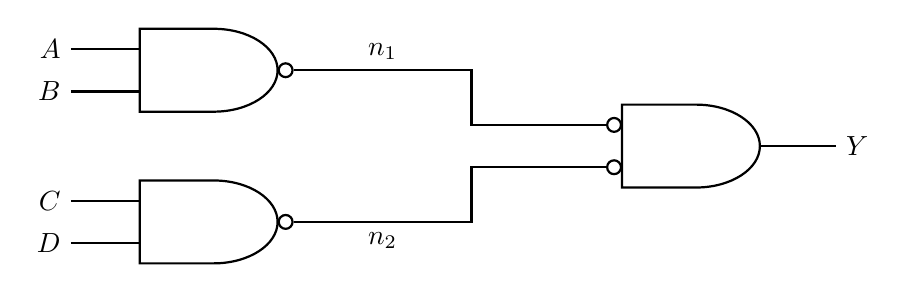
\begin{tikzpicture}[x=1.25cm,y=1.12cm,thick,
      inversion/.style={draw,circle,inner sep=0pt,minimum size=5pt}]
    \foreach \level/\first/\second/\branch in {0.86/A/B/upper,-0.86/C/D/lower} {
      \draw (1.18,{\level-0.47}) -- (1.18,{\level+0.47})
        -- (1.93,{\level+0.47})
        arc[start angle=90,end angle=-90,x radius=0.65,y radius=0.47]
        -- cycle;
      \draw (0.48,{\level+0.24}) node[left] {\(\first\)} -- (1.18,{\level+0.24})
        (0.48,{\level-0.24}) node[left] {\(\second\)} -- (1.18,{\level-0.24});
      \node[inversion,anchor=west] (\branch) at (2.58,\level) {};
    }
    \draw (6.08,-0.47) -- (6.08,0.47) -- (6.83,0.47)
      arc[start angle=90,end angle=-90,x radius=0.65,y radius=0.47]
      -- cycle;
    \node[inversion,anchor=east] (invertUpper) at (6.08,0.24) {};
    \node[inversion,anchor=east] (invertLower) at (6.08,-0.24) {};
    \draw (upper.east) -- (4.55,0.86) node[midway,above] {\(n_1\)}
      |- (invertUpper.west);
    \draw (lower.east) -- (4.55,-0.86) node[midway,below] {\(n_2\)}
      |- (invertLower.west);
    \draw (7.48,0) -- (8.25,0) node[right] {\(Y\)};
  \end{tikzpicture}
  \end{latin}
  \caption{مدار مثال اسلاید ۱۶ با گره‌های میانی \(n_1\) و \(n_2\).
    حباب روی هر پایه مقدار منطقی آن پایه را وارونه می‌کند.
    بازترسیم از اسلاید ۱۶ \cite{powerslides}.}
  \label{fig:power-slide-and-activity}
\end{figure}

دو گیت سمت چپ در خروجی حباب دارند، پس \lr{NAND} هستند.
گیت سمت راست به‌دلیل حباب‌های ورودی، ابتدا هر دو ورودی را
وارونه می‌کند و سپس \lr{AND} می‌گیرد. بنابراین \(Y\) تنها
هنگامی یک می‌شود که \(n_1\) و \(n_2\) هر دو صفر باشند.
این وضعیت دقیقاً زمانی رخ می‌دهد که هر چهار ورودی اولیه یک باشند
\cite[مثال ۵.۲ و شکل \secnum{۵.۹}، صفحات ۱۸۷ و ۱۸۸]{weste}.

فرض می‌کنیم چهار ورودی در هر دوره مستقل و هم‌احتمال‌اند،
بردار ورودی بین دوره‌های متوالی مستقل است و گره‌ها میان
نمونه‌ها گذار اضافی ندارند. پس برای هر ورودی \(p=1/2\)
و \(\alpha=(1/2)(1/2)=1/4\) است. گره \(n_1\) فقط با یک بودن
هم‌زمان \(A\) و \(B\) صفر می‌شود. احتمال آن حالت
\((1/2)(1/2)=1/4\) است. برای \(n_2\)، زوج \(C,D\) همین نقش را
دارد. پس احتمال یک بودن و فعالیت هر گره میانی چنین است.
\[
  p_{n_1}=p_{n_2}=1-\frac14=\frac34,\qquad
  \alpha_{n_1}=\alpha_{n_2}=\frac14\times\frac34=\frac{3}{16}.
\]
دو گره میانی از دو زوج مستقل ورودی ساخته شده‌اند. بنابراین برای
احتمال صفر بودن هم‌زمان آن‌ها، دو احتمال \(1/4\) را در هم ضرب
می‌کنیم. نتیجه با شمارش چهار ورودی هم به دست می‌آید. تنها ترکیب
\((1,1,1,1)\) از میان ۱۶ ترکیب هم‌احتمال، \(Y=1\) می‌دهد.
با اعمال رابطه \eqref{eq:power-activity-independent} بر خروجی داریم.
\[
  p_Y=\frac14\times\frac14=\frac{1}{16},\qquad
  \alpha_Y=\frac{15}{16}\times\frac{1}{16}=\frac{15}{256}.
\]
اگر گره \(n_1\) را وارونه کنیم، احتمال یک بودن از \(3/4\) به
\(1/4\) می‌رسد. در محاسبه فعالیت فقط جای دو عامل
\(p\) و \(1-p\) عوض می‌شود و حاصل همان \(3/16\) است.

% !TeX root = ../complete.tex
\section{کاهش \lr{Switching Power}}
\label{sec:power-dynamic-reduction}

از رابطه \eqref{eq:power-switching} چهار کمیت برای کاهش توان به دست
می‌آیند. توان با \(\alpha\)، \(C_L\) و \(f\) متناسب است و با
مربع \(V_{DD}\) تغییر می‌کند. شرط این مقایسه آن است که هنگام تغییر
هر کمیت، بقیه ثابت باشند. در طراحی واقعی، تغییر ظرفیت یا ولتاژ می‌تواند
تأخیر مسیر را نیز تغییر دهد. پس بعد از برآورد توان، باید معتبر بودن
فرض‌ها و برقراری محدودیت زمانی را بررسی کرد
\cite[بخش \secnum{۵.۲}، صفحات ۱۸۵ تا ۱۹۳]{weste}
\cite[اسلایدهای ۱۳ و ۱۷ تا ۱۹]{powerslides}.

\subsection{توقف ساعت یک بلوک بی‌کار}
\label{sec:power-clock-gating}

\lr{Register} یک یا چند بیت را نگه می‌دارد. در این مثال، در هر لبه
صعودی ساعت، داده ورودی را می‌گیرد و تا لبه بعد نگه می‌دارد. اگر
\lr{Register} ورودی یک بلوک در چند چرخه به‌روزرسانی لازم نداشته باشد،
با \lr{Clock Gating} می‌توان لبه‌های ساعتِ همان بلوک را در آن مدت
متوقف کرد. در این حالت هم گذارهای شاخه ساعت و هم گذارهایی که از
تغییر خروجی این \lr{Register} ناشی می‌شوند، کاهش می‌یابند. اگر
ورودی‌های دیگری مستقل از آن \lr{Register} تغییر کنند، ممکن است بخشی
از منطق بلوک همچنان گذار داشته باشد
\cite[بخش \secnum{۵.۲.۱.۱}، صفحه ۱۸۶]{weste}
\cite[اسلاید ۱۷]{powerslides}.

برای فهم مدار، ساعت اصلی را \(\mathrm{clk}\)، سیگنال اجازه عبور را
\(e\) و ساعت بلوک را \(\mathrm{gclk}\) بنامید. در مدل منطقی،
\(\mathrm{gclk}=\mathrm{clk}\land e\) است. وقتی \(e=1\)، ساعت
بلوک از ساعت اصلی پیروی می‌کند و وقتی \(e=0\)، ساعت بلوک صفر
می‌ماند. اگر \(e\) در میانه سطح بالای ساعت تغییر کند، این گیت
می‌تواند پالس را کوتاه کند یا لبه‌ای ناخواسته به \lr{Register}
بفرستد. راه شکل \secnum{۵.۷} کتاب استفاده از \lr{Latch} است،
یعنی عنصر حافظه‌ای که وقتی ساعت صفر است مقدار اجازه عبور را می‌پذیرد
و در تمام زمان یک‌بودن ساعت آن را ثابت نگه می‌دارد
\cite[شکل \secnum{۵.۷}، صفحه ۱۸۶]{weste}.

اگر یک شاخه در ۱۰ دوره کامل ساعت اصلی تنها چهار دوره پالس داشته
باشد، \(\alpha\) آن شاخه نسبت به ساعت اصلی \(4/10=0.4\) است.
با ثابت بودن ولتاژ و ظرفیت شاخه، توان سوئیچینگ این شاخه ۴۰ درصد
حالت بدون \lr{Clock Gating} می‌شود. اندازه‌گیری صرفه‌جویی کل بلوک
به فعالیت داده‌ها، مصرف مدار کنترل و اجزایی که همچنان ساعت می‌گیرند
نیز وابسته است. تغذیه مدار در این روش وصل می‌ماند.

\subsection{کاهش ظرفیت و کنترل تأخیر}
\label{sec:power-capacitance-reduction}

کوتاه کردن سیمِ گره‌هایی که زیاد سوئیچ می‌کنند، سهم ظرفیت سیم را در
رابطه \eqref{eq:power-node-sum} کم می‌کند. کوچک کردن یک گیت، ظرفیت
ورودی آن را برای مرحله پیشین و ظرفیت \lr{Diffusion} خود گیت را نیز
کم می‌کند. در عوض، گیت کوچک‌تر معمولاً همان بار بعدی را کندتر شارژ
می‌کند. در یک مسیر، اثر هر تغییر را روی ظرفیت، تأخیر مراحل پیش و پس
از گیت و فعالیت گره‌ها بررسی می‌کنیم. مبنای بررسی تأخیر همان
\NotesTopic{sec:delay-path-model}{مدل مسیر در \lr{Logical Effort}}
است \cite[بخش \secnum{۵.۲.۲}، صفحات ۱۸۸ تا ۱۹۰]{weste}
\cite[اسلاید ۱۸]{powerslides}.

برای یک سیم بلند، یکی از گزینه‌ها این است که یک
\lr{Inverter} یا \lr{Buffer} در ابتدای سیم قرار دهیم تا
ظرفیت بزرگ سیم مستقیماً به خروجی گیت منطقی تحمیل نشود. در این
آرایش، گیت منطقی ورودی مرحله جدید را راه‌اندازی می‌کند و
مرحله جدید سیم را شارژ و تخلیه می‌کند. با افزایش اندازه
\lr{Buffer}، بار ورودی آن نیز بیشتر می‌شود. برای تصمیم‌گیری،
ظرفیت ورودی و ظرفیت‌های درونی مرحله اضافه، قطبیت خروجی و تأخیر
کل مسیر را در کنار ظرفیت سیم در نظر می‌گیریم
\cite[بخش \secnum{۵.۲.۲}، صفحه ۱۸۸]{weste}
\cite[اسلاید ۱۸]{powerslides}.

برای نمونه، دو \lr{Inverter} پیاپی با ظرفیت‌های ورودی ۱ و ۴ واحد
و بار نهایی ۱۶ واحد در نظر بگیرید. واحد ظرفیت را ظرفیت ورودی
\lr{Inverter} مرجع و \(\tau\) را واحد تأخیر فصل قبل می‌گیریم.
در مدل عادی‌شده فصل تأخیر، تأخیر هر \lr{Inverter} شامل یک واحد
سهم درونی و نسبت ظرفیت بار به ظرفیت ورودی آن است. با چشم‌پوشی از
ظرفیت سیم و شاخه‌های فرعی، فقط دو گیت داریم. اگر ظرفیت ورودی گیت
دوم را به ۲ واحد برسانیم، تأخیر کل به‌ترتیب قبل و بعد از تغییر چنین است.
\[
  \begin{aligned}
    D_{\mathrm{before}} &= \left(1+\frac{4}{1}\right)
                         +\left(1+\frac{16}{4}\right)=10,\\
    D_{\mathrm{after}}  &= \left(1+\frac{2}{1}\right)
                         +\left(1+\frac{16}{2}\right)=12.
  \end{aligned}
\]
برای تبدیل این اعداد به تأخیر، هرکدام را در \(\tau\) ضرب می‌کنیم.
تأخیر نرمال‌شده گیت اول از ۵ به ۳ کم شده، اما
تأخیر گیت دوم از ۵ به ۹ رسیده است. گیت کوچک‌تر ظرفیت ورودی کم‌تری
دارد و با فرض فعالیت و دامنه یکسان، انرژی شارژ مربوط به همین بخش
از بار گره میانی نصف می‌شود. اگر مهلت مسیر کم‌تر از \(12\tau\)
باشد، این انتخاب با وجود کاهش انرژیِ بار میانی پذیرفتنی نیست.

\subsection{تنظیم ولتاژ و فرکانس}
\label{sec:power-voltage-frequency}

برای مقایسه دو حالت کاریِ یک گره، \(V_1,f_1\) و \(V_2,f_2\)
را ولتاژ و فرکانس حالت‌های اول و دوم بگیرید. اگر ظرفیت و فعالیت
به‌ازای هر دوره ثابت باشند و توان سوئیچینگ حالت اول مثبت باشد، با
تقسیم رابطه \eqref{eq:power-switching} برای دو حالت، عامل‌های مشترک
ساده می‌شوند و نسبت زیر به دست می‌آید.
\begin{equation}
  \frac{P_{\mathrm{sw},2}}{P_{\mathrm{sw},1}}
    =\left(\frac{V_2}{V_1}\right)^2\frac{f_2}{f_1}.
  \label{eq:power-voltage-frequency-ratio}
\end{equation}
مثلاً اگر ولتاژ به ۸۰ درصد و فرکانس به نصف مقدار اولیه برسد، نسبت
توان \(0.8^2\times0.5=0.32\) می‌شود. برای یک کار با تعداد دوره
ثابت، نصف شدن فرکانس زمان انجام کار را دو برابر می‌کند. در این مثال
نسبت انرژی سوئیچینگِ آن کار \(0.32\times2=0.64\) است. اگر ولتاژ
ثابت بماند، کاهش فرکانس به‌تنهایی توان سوئیچینگ را کم می‌کند، ولی
با همین فرض‌ها انرژی سوئیچینگِ کار ثابت می‌ماند. نتیجه به مؤلفه
سوئیچینگ محدود است و انرژی نشتی در زمان اجرای طولانی‌تر می‌تواند
تغییر کند \cite[بخش‌های \secnum{۵.۲.۳} و \secnum{۵.۲.۴}،
صفحات ۱۹۰ تا ۱۹۳]{weste}.

ولتاژ کم‌تر معمولاً جریان راه‌اندازی را کم و گذار را کندتر می‌کند.
ساعت را باید چنان انتخاب کرد که مدار با این تأخیر هنوز کار را در
زمان مقرر انجام دهد. در \lr{Dynamic Voltage and Frequency Scaling}
یا \lr{DVFS}، این دو کمیت برحسب نیاز عملکردیِ بار کاری تنظیم
می‌شوند. در طراحی با \lr{Voltage Domain}، هر بلوک می‌تواند تغذیه
مختص خود را داشته باشد. وقتی سیگنالی از تغذیه کم‌تر به بیش‌تر می‌رود،
سطح یکِ فرستنده ممکن است برای خاموش‌کردن کامل \lr{pMOS} گیرنده
کافی نباشد. \lr{Level Converter} دامنه سیگنال را برای بلوک گیرنده
بازسازی می‌کند. زمان و انرژی خود مبدل نیز در مقایسه معماری‌ها سهم
دارند \cite[بخش \secnum{۵.۲.۳}، صفحات ۱۹۰ تا ۱۹۲]{weste}
\cite[اسلاید ۱۹]{powerslides}.

در \lr{Resonant Clock}، کتاب راه دیگری را برای بار دوره‌ای معرفی
می‌کند. انرژی میان خازن و سلف، یعنی عنصری که انرژی را در میدان
مغناطیسی ذخیره می‌کند، مبادله می‌شود. راه‌انداز در هر دوره انرژی
ازدست‌رفته در مقاومت‌ها را جبران می‌کند. این تغییر مسیر انرژی، فرض
مدل معمول شارژ از منبع و تخلیه کامل به زمین را عوض می‌کند. در برابر
امکان کاهش مصرف، مدار به اجزای بیشتر و فرکانس کاری متناسب با
شبکه تشدید نیاز دارد \cite[بخش \secnum{۵.۲.۶}، صفحه ۱۹۳]{weste}.

% !TeX root = ../complete.tex
\section{مسیرهای جریان و برآورد \lr{Static Power}}
\label{sec:power-static}

\subsection{مصرف توان در یک وضعیت منطقی ثابت}
\label{sec:power-static-sources}

در مدل \lr{Switch} یک گیت مکمل \lr{CMOS}، پس از پایان گذار، یکی
از شبکه‌های \lr{Pull-up} یا \lr{Pull-down} خاموش است و مسیر مستقیم
روشنی میان تغذیه و زمین وجود ندارد. خازن خروجی نیز پس از رسیدن به
ولتاژ نهایی جریان شارژ نمی‌گیرد. در ترانزیستور واقعی، حتی در این وضعیت
جریان‌های کوچک از چند مسیر عبور می‌کنند. برای تغذیه ثابت، اگر این
جریان‌ها سهم‌های جداگانه‌ی جریان کشیده‌شده از همان تغذیه باشند، برآورد
توان ساکن از رابطه زیر به دست می‌آید
\cite[رابطه \secnum{۵.۱۲} و بخش \secnum{۵.۳.۱}،
صفحات ۱۸۵ و ۱۹۴ تا ۱۹۷]{weste}\cite[اسلایدهای ۱۰ و ۲۰]{powerslides}.
\begin{equation}
  P_{\mathrm{stat}}
    =V_{DD}\bigl(I_{\mathrm{sub}}+I_{\mathrm{gate}}+
                 I_{\mathrm{junct}}+I_{\mathrm{cont}}
           \bigr).
  \label{eq:power-static}
\end{equation}
هر جمله داخل پرانتز جریان است و ضرب جمع جریان‌ها در ولتاژ، توان
را برحسب وات می‌دهد. مسیرهای فیزیکی نشتی در
\NotesTopic{sec:leakage}{فصل مدل ترانزیستور} بررسی شده‌اند. در اینجا
اثر هر مسیر را بر جریان کشیده‌شده از منبع دنبال می‌کنیم.

\begin{itemize}
  \item \(I_{\mathrm{sub}}\) سهم \lr{Subthreshold Leakage} است.
    زیر آستانه، ترانزیستور خاموش هنوز می‌تواند جریان کوچکی از مسیر
    کانال عبور دهد. ولتاژهای پایانه‌ها و دما بر این جریان اثر دارند.
    در چند ترانزیستور خاموشِ سری، ولتاژ گره میانی از تعادل جریان
    به دست می‌آید و بایاس هر ترانزیستور با حالت تک‌ترانزیستور فرق
    می‌کند. کاهش نشتی حاصل در بسیاری از وضعیت‌های ورودی را
    \lr{Stack Effect} می‌نامیم.
  \item \(I_{\mathrm{gate}}\) سهم \lr{Gate Leakage} است. اختلاف
    پتانسیل در دو سوی دی‌الکتریک نازک گیت می‌تواند موجب عبور حامل‌ها
    به‌واسطه‌ی \lr{Tunneling} شود. ضخامت و جنس دی‌الکتریک و ولتاژ
    دو سوی آن تعیین می‌کنند این سهم چقدر باشد.
  \item \(I_{\mathrm{junct}}\) سهم \lr{Junction Leakage} است.
    ناحیه‌های \lr{Source} و \lr{Drain} با \lr{Body} پیوند تشکیل
    می‌دهند. حتی یک پیوند با بایاس معکوس جریان کوچکی دارد. میدان
    زیاد نزدیک پیوند می‌تواند سهم سازوکارهایی مانند
    \lr{Band-to-Band Tunneling} را بیشتر کند.
  \item \(I_{\mathrm{cont}}\) سهم \lr{Contention Current} است.
    برای نمونه، در \lr{Pseudo-nMOS} یک \lr{pMOS} همیشه روشن
    خروجی را به سمت تغذیه می‌کشد. هنگامی که شبکه \lr{nMOS} خروجی
    را پایین نگه می‌دارد، هر دو مسیر هم‌زمان هدایت می‌کنند و جریان
    ماندگار برقرار است. این جریان در مدل ماندگار گیت مکمل
    \lr{CMOS} وجود ندارد. \lr{Short-Circuit Current} بخش
    \ref{sec:power-short-circuit} پالس جریان در زمان گذار است.
\end{itemize}

\subsection{برآورد نشتی از عرض افزاره‌ها}
\label{sec:power-static-estimate}

وقتی مقدار یک نشتی به‌ازای واحد عرض معلوم باشد، نخست ترانزیستورها
را برحسب نوع و وضعیت بایاس گروه‌بندی می‌کنیم. در هر گروه، تعداد
افزاره‌ها ضرب‌در عرض متوسط، عرض کل گروه را می‌دهد. اگر کسری از
عرض کل در وضعیت دارای نشتی موردنظر باشد، همان کسر را در عرض کل
و جریان بر واحد عرض ضرب می‌کنیم. برای مثال، در مدل ساده‌ی نشتی
زیرآستانه، \(W_g\) عرض کل گروه \(g\)، \(b_g\) کسر عرضِ خاموش
و \(j_{\mathrm{off},g}\) جریان خاموش بر واحد عرض آن گروه است.
\cite[بخش \secnum{۵.۳.۱.۵}، صفحه ۱۹۷]{weste}
\begin{equation}
  I_{\mathrm{sub}}\approx\sum_g b_g W_g j_{\mathrm{off},g}.
  \label{eq:power-width-leakage}
\end{equation}
\(b_g\) بی‌بعد است. اگر \(W_g\) برحسب میکرومتر و
\(j_{\mathrm{off},g}\) برحسب نانوآمپر بر میکرومتر باشد، حاصل ضرب
برحسب نانوآمپر خواهد بود. ثبات مقدار جریان بر واحد عرض در هر گروه
یک تقریب است. به‌ویژه، جدول \secnum{۵.۲} کتاب نشان می‌دهد که در
یک \lr{NAND} سه‌ورودی، تغییر ترتیب ورودی‌ها می‌تواند ولتاژ گره‌های
میانی و درنتیجه نشتی را عوض کند \cite[صفحه ۱۹۶]{weste}.

در مثال ۵.۴ کتاب و اسلایدهای ۲۱ و ۲۲، دوباره همان تراشه‌ی بخش
\ref{sec:power-effective-capacitance} را بررسی می‌کنیم. از ۵۰ میلیون
ترانزیستور منطق با عرض متوسط \qty{0.30}{\micro\metre}، سهم
۵ درصد در گروه با آستانه پایین‌تر و ۹۵ درصد در گروه آستانه بالا
قرار می‌گیرند. اسلاید گروه ۵ درصدی را \lr{Normal \(V_t\)} و
کتاب در مثال ۵.۴ آن را \lr{low-threshold} می‌نامد. هر دو منبع
برای این گروه در حالت خاموش، مقدار
\qty[per-mode=symbol]{100}{\nano\ampere\per\micro\metre}
به کار می‌برند. \(W_{\mathrm{nom}}\) عرض کل این گروه و
\(W_{\mathrm{high}}\) عرض کل گروه آستانه بالاست.
همه‌ی ۹۵۰ میلیون ترانزیستور حافظه با عرض متوسط
\qty{0.10}{\micro\metre} در گروه آستانه بالا قرار می‌گیرند.
عرض کل دو گروه از جمع عرض ترانزیستورهایشان به دست می‌آید
\cite[مثال ۵.۴، صفحه ۱۹۷]{weste}\cite[اسلایدهای ۲۱ و ۲۲]{powerslides}.
\[
  \begin{aligned}
    W_{\mathrm{nom}}&=(50\times10^6)(0.05)
                       (\qty{0.30}{\micro\metre})
                     =\qty{0.75e6}{\micro\metre},\\
    W_{\mathrm{high}}&=(50\times10^6)(0.95)
                        (\qty{0.30}{\micro\metre})
                        +(950\times10^6)(\qty{0.10}{\micro\metre})\\
                    &=\qty{109.25e6}{\micro\metre}.
  \end{aligned}
\]
در این برآورد، نصف عرض هر گروه در حالت خاموش است. \lr{Stack Effect}
را کنار می‌گذاریم و با مقادیر خاموشِ داده‌شده در مثال، سهم کانال را
حساب می‌کنیم. برای سهم گیت فرض می‌کنیم نیمه‌ی روشنِ عرض کل دارای
آن نشتی است. پس نصف مجموع عرض را در
\qty[per-mode=symbol]{5}{\nano\ampere\per\micro\metre} ضرب می‌کنیم.
\[
  \begin{aligned}
    I_{\mathrm{sub}} &\approx \tfrac12\bigl[
       W_{\mathrm{nom}}(\qty[per-mode=symbol]{100}{\nano\ampere\per\micro\metre})
      +W_{\mathrm{high}}(\qty[per-mode=symbol]{10}{\nano\ampere\per\micro\metre})
      \bigr]\approx\qty{584}{\milli\ampere},\\
    I_{\mathrm{gate}}&\approx\tfrac12(W_{\mathrm{nom}}+W_{\mathrm{high}})
        (\qty[per-mode=symbol]{5}{\nano\ampere\per\micro\metre})
        =\qty{275}{\milli\ampere}.
  \end{aligned}
\]
با فرض ناچیز بودن نشتی پیوند و نبود مسیر ماندگار ناشی از هدایت
هم‌زمان، جمع این دو جریان در تغذیه \qty{1.0}{\volt} حدود
\qty{859}{\milli\watt} توان ساکن می‌دهد. این مقدار در همان مدل
تراشه حتی اگر ساعت متوقف شود و وضعیت بایاس و دما ثابت بمانند،
با صفر شدن توان سوئیچینگ از بین نمی‌رود. نسبت آن به برآورد
\qty{6.1}{\watt} سوئیچینگ بخش \ref{sec:power-effective-capacitance}
حدود ۱۴ درصد است. هر دو برآورد به داده‌ها و فرض‌های همین مثال
وابسته‌اند.

\subsection{کاهش نشتی با انتخاب افزاره و وضعیت ورودی}
\label{sec:power-leakage-controls}

مقدار \(V_t\) تعیین می‌کند ترانزیستور در یک ولتاژ گیت معین چه
مقدار جریان عبور می‌دهد. با ثابت بودن سایر بایاس‌ها و دما، بالا بردن
آستانه به اندازه \(\Delta V_t\) جمله نماییِ جریان زیرآستانه را
در مدل فصل ۲ در عامل زیر ضرب می‌کند. \(S\) تغییر ولتاژ لازم برای
یک دهه تغییر جریان است
\cite[بخش‌های \secnum{۲.۴.۴} و \secnum{۵.۳.۱.۱}]{weste}.
\[
  \frac{I_{\mathrm{sub,new}}}{I_{\mathrm{sub,old}}}
  \approx 10^{-\Delta V_t/S}.
\]
برای مثال، اگر \(S\) برابر \qty{100}{\milli\volt} بر دهه باشد،
افزایش \qty{50}{\milli\volt} آستانه، نمای کسر را به \(-1/2\)
می‌رساند. \(10^{-1/2}=1/\sqrt{10}\) است، پس جریان تخمینی به حدود
۳۲ درصد مقدار اولیه می‌رسد. مقدار \(S\) و جریان اولیه از بایاس، دما
و فناوری می‌آیند.

در کتابخانه دارای چند آستانه، \lr{High-\(V_t\)} برای مسیر دارای
مهلت کافی، نشتی زیرآستانه‌ی کمتری دارد. \lr{Low-\(V_t\)} در بخش
حساس به تأخیر می‌تواند جریان روشن بیشتری بدهد. دی‌الکتریک ضخیم‌تر
در فناوری‌هایی که آن گزینه را دارند، می‌تواند نشتی گیت را کم کند.
سرعت و سازگاری سلول با ولتاژ کاری هنگام انتخاب هر نوع بررسی می‌شوند
\cite[بخش \secnum{۵.۳.۳}، صفحه ۱۹۹]{weste}.

در \lr{Body Bias}، ولتاژ \lr{Body} نسبت به \lr{Source} تنظیم
می‌شود. در \lr{nMOS}، افزایش بایاس معکوس پیوند بدنه و سورس در
محدوده معتبر مدل، آستانه را بالا می‌برد و می‌تواند جریان زیرآستانه
را کم کند. بایاس معکوس زیاد، میدان پیوند را افزایش می‌دهد و ممکن
است نشتی پیوند بیشتر شود. با \lr{Input Vector Control} نیز می‌توان
هنگام بی‌کاری ترکیبی از ورودی‌ها را اعمال کرد که وضعیت ترانزیستورهای
خاموش در شاخه‌های سری نشتی کمتری ایجاد کند. هزینه تغییر ورودی‌ها
و صرفه‌جویی در طول بی‌کاری هر دو در ارزیابی این روش سهم دارند
\cite[بخش‌های \secnum{۵.۳.۴} و \secnum{۵.۳.۵}،
صفحات ۱۹۹ و ۲۰۰]{weste}.

% !TeX root = ../complete.tex
\section{قطع تغذیه بلوک با \lr{Power Gating}}
\label{sec:power-gating}

\subsection{مسیر تغذیه، جداسازی خروجی و حفظ وضعیت}
\label{sec:power-gating-operation}

در \NotesTopic{sec:power-clock-gating}{\lr{Clock Gating}}، ساعت
بلوک متوقف می‌شود و ریل تغذیه به مدار وصل می‌ماند. در \lr{Power Gating}،
یک ترانزیستور سری، مسیر تغذیه بلوک را در حالت خواب قطع می‌کند.
در شکل \ref{fig:power-gating-header}، یک \lr{pMOS Header} میان
تغذیه اصلی \(V_{DD}\) و ریل تغذیه بلوک قرار دارد. ولتاژ ریل بعد
از کلید را \(V_{DDV}\) می‌نامیم. آن را ریل تغذیه مجازی می‌گویند،
زیرا مقدارش به وضعیت کلید، بار و نشتی بلوک وابسته است. گزینه‌ی دیگر
\lr{nMOS Footer} است که به‌جای تغذیه بالا، مسیر اتصال به زمین را
قطع می‌کند \cite[بخش \secnum{۵.۳.۲}، صفحات ۱۹۷ و ۱۹۸]{weste}
\cite[اسلاید ۲۳]{powerslides}.

\begin{figure}[htbp]
  \centering
  \begin{latin}
  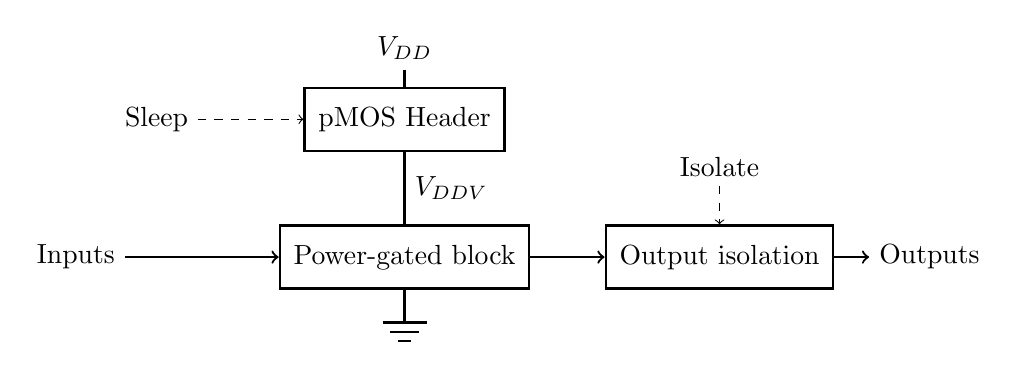
\begin{tikzpicture}[
    x=1cm,y=1cm,
    component/.style={draw,thick,minimum height=8mm,align=center,inner sep=5pt}
  ]
    \node[component] (header) at (0,1.75) {pMOS Header};
    \node[component] (block) at (0,0) {Power-gated block};
    \node[component] (isolate) at (4,0) {Output isolation};
    \node (supply) at (0,2.65) {\(V_{DD}\)};
    \node (sleep) at (-3.15,1.75) {Sleep};
    \node (clamp) at (4,1.15) {Isolate};
    \draw[thick] (supply) -- (header.north);
    \draw[thick] (header.south) -- (block.north)
      node[midway,right] {\(V_{DDV}\)};
    \draw[dashed,->] (sleep.east) -- (header.west);
    \draw[dashed,->] (clamp.south) -- (isolate.north);
    \draw[->,thick] (-3.55,0) node[left] {Inputs} -- (block.west);
    \draw[->,thick] (block.east) -- (isolate.west);
    \draw[->,thick] (isolate.east) -- (5.9,0) node[right] {Outputs};
    \draw[thick] (block.south) -- (0,-0.83);
    \draw[thick] (-0.28,-0.83) -- (0.28,-0.83);
    \draw[thick] (-0.18,-0.95) -- (0.18,-0.95);
    \draw[thick] (-0.08,-1.07) -- (0.08,-1.07);
  \end{tikzpicture}
  \end{latin}
  \caption{مسیر تغذیه و مسیر داده در یک بلوک دارای \lr{Power Gating}.
    \lr{Sleep} کلید تغذیه را کنترل می‌کند و \lr{Isolate} سطح خروجی را
    هنگام قطع تغذیه معتبر نگه می‌دارد. طرح مفهومی از شکل \secnum{۵.۲۴}
    کتاب و اسلاید ۲۳ اقتباس شده است \cite{weste,powerslides}.}
  \label{fig:power-gating-header}
\end{figure}

در حالت فعال، کلید روشن است و ریل مجازی نزدیک \(V_{DD}\) می‌ماند.
در خواب، کلید خاموش می‌شود و بار ذخیره‌شده روی ریل مجازی می‌تواند
از مسیرهای نشتی کاهش یابد. تا زمانی که تغذیه بلوک دوباره برقرار شود،
خروجی آن ممکن است در محدوده نامعتبر بین صفر و یک بماند. مدار
\lr{Output Isolation} با تغذیه برقرار، پیش از قطع تغذیه خروجی را
به یک سطح مشخص مانند صفر محدود می‌کند. اگر بلوک باید پس از بیداری
از همان داده ادامه دهد، داده را در \lr{Retention Register} با تغذیه
برقرار یا در حافظه‌ای بیرون از دامنه‌ی خاموش نگه می‌دارند. پس از
وصل تغذیه، ریل فرصت بازیابی دارد و وضعیت لازم بازیابی یا مقداردهی
اولیه می‌شود. جداسازی هنگامی برداشته می‌شود که خروجی‌های بلوک معتبر
باشند \cite[بخش \secnum{۵.۳.۲}، صفحات ۱۹۷ تا ۱۹۹]{weste}.

\subsection{افت روی کلید و اثر آن بر تأخیر}
\label{sec:power-header-delay}

در یک برآورد دست‌اول برای کلید روشن، \(W\) عرض مؤثر کلید،
\(R_h\) مقاومت روشن و \(r_w\) حاصل‌ضرب مقاومت روشن در عرض است.
\(r_w\) برای طول کانال و شرایط بایاس مشخص داده می‌شود و می‌توان آن
را با اهم‌میکرومتر بیان کرد. اگر جریان نماینده‌ی بلوک در حالت فعال
\(I_{\mathrm{on}}\) باشد، قانون اهم افت ریل را به عرض کلید ربط می‌دهد.
\begin{equation}
  R_h\approx\frac{r_w}{W},\qquad
  \Delta V=V_{DD}-V_{DDV}\approx I_{\mathrm{on}}R_h.
  \label{eq:power-header-droop}
\end{equation}
ضرب آمپر در اهم واحد ولت دارد. بزرگ‌تر کردن عرض، در این مدل
مقاومت و افت را کاهش می‌دهد. به‌کارگیری جریان متوسط برای بلوک بزرگ
هنگامی مناسب‌تر است که رویدادهای سوئیچینگ در زمان پخش شوند و ظرفیت
روی ریل مجازی، نوسان ولتاژ را هموار کند. اگر چند بار هم‌زمان جریان
زیادی بکشند، افت گذرا می‌تواند با برآورد متوسط تفاوت داشته باشد
\cite[بخش \secnum{۵.۳.۲.۱}، صفحات ۱۹۸ و ۱۹۹]{weste}.

برای مرتبط کردن افت ریل با تأخیر، \(V\) را ولتاژ مؤثر تغذیه بلوک،
\(V_t>0\) را آستانه‌ی مؤثر و \(D(V)\) را تأخیر مسیر در آن ولتاژ
می‌گیریم. برآورد فصل ۳ از تقسیم بار جابه‌جاشده بر جریان شروع می‌شود.
برای تغییر ولتاژ به اندازه‌ی کسری ثابت از \(V\)، بار با \(V\) متناسب
است. در \lr{Alpha-Power Law} جریان راه‌اندازی با \((V-V_t)^m\)
متناسب است. توان تجربی \(m\) معمولاً بین ۱ و ۲ است. کتاب آن را
\(\alpha\) می‌نویسد. در این فصل، \(\alpha\) برای \lr{Activity Factor}
به کار می‌رود. اگر ظرفیت و پارامترهای مدل ثابت باشند، برای \(V>V_t\)
با ثابت مثبت \(K\) داریم
\cite[رابطه \secnum{۴.۲۹}، صفحه ۱۶۲]{weste}.
\begin{equation}
  D(V)=K\frac{V}{(V-V_t)^m}.
  \label{eq:power-above-threshold-delay}
\end{equation}
\(K\) ظرفیت، ضرایب جریان و عوامل ثابت مربوط به مسیر را در بر می‌گیرد.
در این نوشتار، واحد آن \(\mathrm{s}\,\mathrm{V}^{m-1}\) است تا پس
از ضرب در \(V/(V-V_t)^m\)، حاصل واحد زمان داشته باشد. با تقسیم تأخیر ریل
مجازی بر تأخیر اولیه، \(K\) حذف می‌شود و نسبت زیر از مدل به دست می‌آید.
\begin{equation}
  \frac{D(V_{DD}-\Delta V)}{D(V_{DD})}
    =\left(1-\frac{\Delta V}{V_{DD}}\right)
      \left(\frac{V_{DD}-V_t}{V_{DD}-V_t-\Delta V}\right)^m.
  \label{eq:power-droop-delay-ratio}
\end{equation}
این نسبت برای \(0\leq\Delta V<V_{DD}-V_t\) تعریف شده است. اگر
افت صفر باشد، نسبت یک است. برای افت مثبت، عامل نخست کم‌تر از یک
و عامل دوم بزرگ‌تر از یک است. در این مدل با \(m\geq 1\)، کاهش
توانایی جریان‌دهی بر کاهش بار لازم برای گذار غلبه می‌کند.

برای افت کوچک می‌توان از حساسیت تأخیر استفاده کرد. اگر مقدار ولتاژ
از \(V\) به \(V-\Delta V\) برود، تقریب خطیِ تابع نزدیک \(V\)
می‌دهد \(D(V-\Delta V)-D(V)\approx-D'(V)\Delta V\).
برای محاسبه مشتق، \(D(V)=KV(V-V_t)^{-m}\) را به‌شکل ضرب دو
تابع می‌نویسیم. مشتق عامل اول \(K\) است. برای مشتق عامل دوم، قاعده
توان، \(-m(V-V_t)^{-m-1}\) را می‌دهد و طبق قاعده زنجیره‌ای آن را
در مشتق \(V-V_t\)، یعنی یک، ضرب می‌کنیم. حاصلِ قاعده ضرب پس از تقسیم بر
\(D(V)\)، دو جمله برای حساسیت باقی می‌گذارد. با \(V=V_{DD}\)
و \(\Delta D=D(V_{DD}-\Delta V)-D(V_{DD})\)، نتیجه چنین است.
\begin{equation}
  \frac{\Delta D}{D(V_{DD})}
  \approx\left(\frac{m}{V_{DD}-V_t}-\frac{1}{V_{DD}}\right)\Delta V.
  \label{eq:power-droop-delay-sensitivity}
\end{equation}
عبارت داخل پرانتز واحد معکوس ولت دارد و حاصل بی‌بعد است. هرچه
\(V_{DD}-V_t\) کوچک‌تر باشد، افت معین می‌تواند اثر نسبی بیشتری
بر تأخیر بگذارد. برای نمونه، با \(V_t/V_{DD}=0.30\) و \(m=1.4\)
عبارت داخل پرانتز \(1/V_{DD}\) است و در تقریب خطی درصد افزایش
تأخیر با درصد افت تغذیه برابر می‌شود. برابری درصدها به پارامترها
و کوچک بودن افت وابسته است.

\subsection{اندازه کلید و حداقل زمان خواب}
\label{sec:power-header-sizing}

اگر حد مجاز افت ریل \(\Delta V_{\max}>0\) معلوم باشد، با جای‌گذاری
\(R_h\) در رابطه \eqref{eq:power-header-droop} و اعمال شرط
\(\Delta V\leq\Delta V_{\max}\)، از مدل مقاومتی حد زیر بر عرض
به دست می‌آید. همه‌ی کمیت‌ها مثبت‌اند و ضرب و تقسیم جهت نامساوی
را تغییر نمی‌دهد.
\begin{equation}
  W\geq\frac{I_{\mathrm{on}}r_w}{\Delta V_{\max}}.
  \label{eq:power-header-width}
\end{equation}
در مثال ۵.۵ کتاب، تغذیه \qty{1}{\volt} و توان فعال میانگین حافظه
\qty{2}{\watt} است. تقسیم توان بر ولتاژ، جریان \qty{2}{\ampere}
را می‌دهد. کتاب برای بررسی افزایش تأخیرِ ۵ درصدی در همان مثال،
افت ریل را تقریباً ۵ درصدِ تغذیه می‌گیرد، یعنی
\qty{50}{\milli\volt}. مقاومت کلید از تقسیم این افت بر جریان
به‌دست می‌آید و حداکثر \qty{25}{\milli\ohm} است. برای
\(r_w=\qty{2}{\kilo\ohm\micro\metre}\) حد عرض چنین می‌شود
\cite[مثال ۵.۵، صفحات ۱۹۸ و ۱۹۹]{weste}.
\[
  W\geq\frac{\qty{2e3}{\ohm\micro\metre}}{\qty{25e-3}{\ohm}}
    =\qty{8e4}{\micro\metre}.
\]
واحد اهم ساده می‌شود و این عرض، مجموع عرض مؤثر کلیدهایی است که
می‌توان موازی بست. کتاب برای همان مثال از شبیه‌سازی مدار عرض کم‌تری
به دست می‌آورد و تفاوت را با تغییر مقاومت روشن در بایاس واقعی توضیح
می‌دهد. هنگام روشن شدن کلید، شارژ ریل مجازی می‌تواند جریان آغازین
بزرگی ایجاد کند. روشن کردن گروه‌های موازی در چند گام، روشی برای
محدود کردن این جریان آغازین است \cite[صفحه ۱۹۹]{weste}.

برای سنجش صرفه‌ی خواب، \(P_{\mathrm{idle}}\) را توان بلوک در حالت
بی‌کارِ دارای تغذیه، \(P_{\mathrm{sleep}}\) را توان بلوک در خواب و
\(E_{\mathrm{tr}}\) را انرژی اضافیِ ورود و خروج از خواب بگیرید.
اگر \(P_{\mathrm{idle}}>P_{\mathrm{sleep}}\)، در مدت خواب \(T_s\)
به‌اندازه‌ی \((P_{\mathrm{idle}}-P_{\mathrm{sleep}})T_s\) انرژی
صرفه‌جویی می‌شود. خواب هنگامی از لحاظ انرژی به‌صرفه است که این مقدار
از \(E_{\mathrm{tr}}\) بیشتر باشد. با حل نامساوی برای زمان، شرط
به صورت زیر است \cite[بخش \secnum{۵.۳.۲}، صفحات ۱۹۷ و ۱۹۸]{weste}.
\begin{equation}
  T_s > T_{\mathrm{BE}}
      =\frac{E_{\mathrm{tr}}}{P_{\mathrm{idle}}-P_{\mathrm{sleep}}}.
  \label{eq:power-gating-break-even}
\end{equation}
\(T_{\mathrm{BE}}\) زمان سربه‌سر انرژی است. ژول تقسیم بر وات
ثانیه می‌دهد. برای نمونه، اگر هزینه تغییر حالت \qty{1}{\nano\joule}
و کاهش توان \qty{2}{\milli\watt} باشد، تقسیم
\qty{1e-9}{\joule} بر \qty{2e-3}{\watt} برابر
\qty{0.5}{\micro\second} است. جدا از صرفه‌ی انرژی، زمان بیداری
نیز باید با مهلت پاسخ سامانه سازگار باشد.

% !TeX root = ../complete.tex
\section{مقایسه انرژی و تأخیر یک عملیات}
\label{sec:power-energy-delay}

\subsection{توان متوسط و انرژی به‌ازای هر عملیات}
\label{sec:power-energy-per-operation}

برای مقایسه دو پیاده‌سازی، ابتدا کاری را که هر دو باید انجام دهند
مشخص می‌کنیم. اگر مدار در بازه‌ای به مدت \(D\) فقط یک عملیات
انجام دهد و توان متوسط در همان مدت \(P_{\mathrm{avg}}\) باشد، از رابطه
\eqref{eq:power-interval}، انرژی عملیات \(E_{\mathrm{op}}=P_{\mathrm{avg}}D\)
به دست می‌آید. اگر توان را در بازه‌ای با چند عملیات اندازه بگیریم،
انرژی کل را بر تعداد عملیات کامل‌شده تقسیم می‌کنیم. با نرخ انجام
عملیات \(r_{\mathrm{op}}\)، یعنی تعداد عملیات کامل‌شده در ثانیه،
انرژی متوسط به‌ازای هر عملیات \(P_{\mathrm{avg}}/r_{\mathrm{op}}\)
است. در این کسر، واحد وات تقسیم بر معکوس ثانیه، ژول می‌دهد.
وقتی میانگین یک نتیجه در هر دوره ساعت باشد،
\(r_{\mathrm{op}}=f\) است. برای کاری که به چند دوره نیاز دارد،
رابطه را با نرخ واقعی انجام کار به کار می‌بریم
\cite[بخش‌های \secnum{۵.۴.۱} و \secnum{۵.۶}، صفحات
۲۰۰ و ۲۰۶]{weste}.

برای برآورد انرژی یک عملیات در تغذیه \(V\)، فرض کنید گره \(i\)
با ظرفیت معادل \(C_i\) در آن عملیات \(N_{\uparrow,i}\) بار از صفر
تا \(V\) شارژ می‌شود. مطابق رابطه \eqref{eq:power-source-energy}،
با جمع انرژی شارژِ همه گره‌ها، انرژی سوئیچینگ به دست می‌آید. مجموع
وزن‌دار \(C_{\mathrm{op}}=\sum_i N_{\uparrow,i} C_i\) واحد ظرفیت
دارد. اگر جریان نشتیِ متوسط \(I_{\mathrm{leak}}\) را برای مدت
انجام کار در نظر بگیریم و سهم پالس جریان مستقیم و هدایت هم‌زمان
ماندگار ناچیز باشند، مدل انرژی چنین است
\cite[رابطه \secnum{۵.۲۵}، صفحه ۲۰۲]{weste}.
\begin{equation}
  E_{\mathrm{op}}\approx E_{\mathrm{sw}}+E_{\mathrm{leak}}
    =C_{\mathrm{op}}V^2+I_{\mathrm{leak}}VD.
  \label{eq:power-operation-energy}
\end{equation}
جمله نخست با شمار شارژها و مربع ولتاژ تغییر می‌کند. در جمله دوم،
\(I_{\mathrm{leak}}V\) توان نشتی است و ضرب آن در مدت انجام کار،
انرژی نشتی را می‌دهد. بنابراین حتی کاهش توان نشتی می‌تواند با
بلندتر شدن زمان انجام کار به افزایش انرژی نشتی بینجامد.

\subsection{کمینه انرژی و کار در ولتاژ پایین}
\label{sec:power-minimum-energy}

در بخش \ref{sec:power-header-delay} از مدل جریان با اضافه‌ولتاژ
مثبت استفاده کردیم. اگر \(V\) پایین‌تر از \(V_t\) باشد، هنوز
جریان زیرآستانه وجود دارد. در تقریب بخش \secnum{۴.۴.۶.۴} کتاب،
جریان راه‌انداز با \(10^{V/S}\) متناسب است. \(S\) همان ولتاژ لازم
برای تغییر ده‌برابری جریان در مدل زیرآستانه است. با ثابت گرفتن
پارامترهای فناوری، ظرفیت مسیر و عوامل دیگری که بر جریان اثر دارند،
تقسیم بار متناسب با \(V\) بر جریان، تخمین زیر را برای مدت انجام
عملیاتِ محدود به یک مسیر می‌دهد
\cite[رابطه‌های \secnum{۴.۳۱} و \secnum{۵.۲۴}،
صفحات ۱۶۲ و ۲۰۲]{weste}.
\begin{equation}
  D(V)\approx K_s\,V\,10^{-V/S}.
  \label{eq:power-subthreshold-delay}
\end{equation}
\(K_s\) یک ضریب مثبت با واحد ثانیه بر ولت است که ظرفیت و ضریب
جریان مسیر را در بر می‌گیرد. اگر \(V\) به‌اندازه \(S\) کاهش
یابد، عامل نمایی ده برابر می‌شود. هم‌زمان، عامل خطی \(V\) کمی
کوچک‌تر می‌شود. در محدوده‌ای که اثر نمایی غالب است، تأخیر به‌سرعت
زیاد می‌شود. این مدل برای مقایسه نقطه‌های کاری معتبر در محدوده
زیرآستانه است. در ولتاژهای بسیار پایین، توانایی مدار در تولید و
حفظ سطوح منطقی نیز باید با معیار فصل ۲ بررسی شود.

برای نمونه، سه ولتاژ کاری زیر آستانه در یک مدل فرضی را مقایسه کنید.
می‌گیریم \(C_{\mathrm{op}}=\qty{20}{\femto\farad}\)،
\(I_{\mathrm{leak}}=\qty{5}{\nano\ampere}\) و
\(S=\qty{0.10}{\volt}\). برای این بازه فرض می‌کنیم تغییر
جریان نشتی با ولتاژ ناچیز است. زمان مرجع \(D_0=\qty{300}{\nano\second}\)
در \(V_0=\qty{0.30}{\volt}\) داده شده و همه‌ی ولتاژهای جدول در
محدوده معتبر مدل فرض می‌شوند. برای انتقال از زمان مرجع به زمان هر
ردیف، رابطه \eqref{eq:power-subthreshold-delay} را در دو ولتاژ بر
هم تقسیم می‌کنیم. حاصل به صورت زیر است.
\[
  \frac{D(V)}{D_0}\approx
    \frac{V}{V_0}\,10^{(V_0-V)/S}.
\]
در \qty{0.20}{\volt}، عامل نمایی ۱۰ و عامل خطی \(2/3\) است.
پس تأخیر تقریباً \((20/3)D_0=\qty{2000}{\nano\second}\) می‌شود.
در \qty{0.40}{\volt}، عامل نمایی \(1/10\) و عامل خطی \(4/3\)
است و تأخیر به \qty{40}{\nano\second} می‌رسد. برای نمونه در
ولتاژ پایین‌تر، جای‌گذاری در رابطه \eqref{eq:power-operation-energy}
دو مؤلفه را چنین می‌دهد.
\[
  \begin{aligned}
    E_{\mathrm{sw}}&=(\qty{20}{\femto\farad})(\qty{0.20}{\volt})^2
                     =\qty{0.80}{\femto\joule},\\
    E_{\mathrm{leak}}&=(\qty{5}{\nano\ampere})(\qty{0.20}{\volt})
                         (\qty{2.0}{\micro\second})
                     =\qty{2.0}{\femto\joule}.
  \end{aligned}
\]
همین محاسبه برای هر سه ولتاژ در جدول \ref{tab:power-energy-candidates}
آمده است. انرژی‌ها تا رقم اعشاری دوم نمایش داده شده‌اند تا جمع و
مقایسه ردیف‌ها روشن باشد.

\begin{table}[htbp]
  \centering
  \caption{انرژی و زمان یک عملیات در سه نقطه کاریِ یک مدل فرضی.
    \(E_{\mathrm{op}}\) از جمع انرژی سوئیچینگ و نشتی به دست آمده است.}
  \label{tab:power-energy-candidates}
  \begin{tabular}{ccccc}
    \toprule
    \(V\,(\unit{\volt})\) & \(D\,(\unit{\nano\second})\) &
    \(E_{\mathrm{sw}}\,(\unit{\femto\joule})\) &
    \(E_{\mathrm{leak}}\,(\unit{\femto\joule})\) &
    \(E_{\mathrm{op}}\,(\unit{\femto\joule})\) \\
    \midrule
    \num{0.20} & \num{2000} & \num{0.80} & \num{2.00} & \num{2.80} \\
    \num{0.30} & \num{300}  & \num{1.80} & \num{0.45} & \num{2.25} \\
    \num{0.40} & \num{40}   & \num{3.20} & \num{0.08} & \num{3.28} \\
    \bottomrule
  \end{tabular}
\end{table}

از میان این سه نقطه، \qty{0.30}{\volt} کم‌ترین انرژی را دارد.
در ولتاژ پایین‌تر، کاهش انرژی سوئیچینگ با افزایش انرژی نشتی در
زمان اجرای طولانی خنثی می‌شود. در ولتاژ بالاتر، انرژی سوئیچینگ
بزرگ‌تر است. این مقایسه کمینه را فقط در مجموعه سه گزینه مشخص
می‌کند. در مدار واقعی، تغییر فعالیت، آستانه یا دما می‌تواند
نقطه کمینه را جابه‌جا کند. این وابستگی در نقشه‌های شکل
\secnum{۵.۲۷} کتاب نیز دیده می‌شود \cite[صفحات ۲۰۲ و ۲۰۳]{weste}.

\subsection{کمینه \lr{Energy--Delay Product}}
\label{sec:power-edp}

گاهی هر دو هزینه انرژی عملیات و زمان اجرای آن در رتبه‌بندی اهمیت
دارند. معیار \lr{Energy--Delay Product} یا \lr{EDP}، حاصل‌ضرب
این دو با واحد ژول‌ثانیه است. محاسبه را برای \(V>V_t>0\) و با
\(C_{\mathrm{op}}>0\)، \(V_t\) و پارامترهای مسیر ثابت انجام می‌دهیم.
اگر انرژی سوئیچینگ غالب باشد، با ضرب انرژیِ رابطه
\eqref{eq:power-operation-energy} در تأخیرِ رابطه
\eqref{eq:power-above-threshold-delay} داریم
\cite[رابطه \secnum{۵.۲۶}، صفحه ۲۰۳]{weste}.
\begin{equation}
  \mathrm{EDP}(V)=E_{\mathrm{op}}(V)D(V)
       \approx K C_{\mathrm{op}}\frac{V^3}{(V-V_t)^m}.
  \label{eq:power-edp}
\end{equation}
برای یافتن کمینه، تغییر \(V^3(V-V_t)^{-m}\) را با ولتاژ بررسی
می‌کنیم. قاعده‌ی ضرب یک جمله از مشتق \(V^3\) و یک جمله از
مشتق \((V-V_t)^{-m}\) می‌دهد. با بیرون کشیدن عامل مشترک، مشتق
مدل \(\mathrm{EDP}\) چنین می‌شود.
\[
  \begin{aligned}
    \frac{\mathrm{d}(\mathrm{EDP})}{\mathrm{d}V}
       &=K C_{\mathrm{op}}\bigl[3V^2(V-V_t)^{-m}
                         -mV^3(V-V_t)^{-m-1}\bigr]\\
       &=K C_{\mathrm{op}} V^2 (V-V_t)^{-m-1}
           \bigl[(3-m)V-3V_t\bigr].
  \end{aligned}
\]
برای \(1\leq m\leq 2\)، عامل بیرون کروشه مثبت و شیب عبارت
خطی داخل کروشه \(3-m>0\) است. مشتق در نقطه‌ای که عبارت داخل
کروشه صفر می‌شود، از منفی به مثبت تغییر می‌کند. بنابراین کمینه
مدل در این ولتاژ است \cite[رابطه \secnum{۵.۲۷}، صفحه ۲۰۳]{weste}.
\begin{equation}
  V_{\mathrm{EDP}}=\frac{3}{3-m}\,V_t.
  \label{eq:power-edp-voltage}
\end{equation}
برای \(m=1.5\)، این ولتاژ دو برابر آستانه‌ است. اگر آستانه
فرضی \qty{0.30}{\volt} باشد، مدل \qty{0.60}{\volt} می‌دهد.
این محاسبه از تقریبِ صرف‌نظر از نشتی استفاده می‌کند. اگر ولتاژ
به گزینه‌های مشخص محدود باشد یا انرژی نشتی قابل‌توجه باشد، باید
انرژی و تأخیر را در گزینه‌های مجاز با مدل مناسب همان شرایط مقایسه کرد.

\subsection{کمینه انرژی با مهلت زمانی مشخص}
\label{sec:power-delay-constraint}

فرض کنید زمان انجام کار باید حداکثر \(D_{\max}\) باشد. ابتدا فقط
گزینه‌هایی را نگه می‌داریم که \(D\leq D_{\max}\) دارند و سپس انرژی
آن‌ها را مقایسه می‌کنیم. برای مثال، با مهلت \qty{100}{\nano\second}
از جدول \ref{tab:power-energy-candidates} فقط گزینه‌ی
\qty{0.40}{\volt} می‌ماند. اگر مهلت به \qty{300}{\nano\second}
برسد، گزینه‌ی \qty{0.30}{\volt} نیز مجاز می‌شود و میان گزینه‌های
مجاز انرژی کم‌تری دارد.

این روش برای مقایسه توپولوژی و اندازه گیت‌ها نیز کاربرد دارد.
در ولتاژ ثابت، از \NotesTopic{sec:delay-path-model}{مدل تأخیر مسیر}
برای یافتن کندترین مسیر هر گزینه و از مجموع ظرفیت‌های وزن‌دار
رابطه \eqref{eq:power-operation-energy} برای برآورد انرژی استفاده
می‌کنیم. همان‌طور که مثال بخش \ref{sec:power-capacitance-reduction}
نشان داد، کاهش اندازه یک گیت ممکن است انرژی را کم و تأخیر مسیر را
زیاد کند. کتاب شکل \secnum{۵.۱۳} را با تکرار همین مسئله برای
مهلت‌های متفاوت به دست می‌آورد. هر نقطه روی آن منحنی، انرژیِ کمینه
مدل با یک مهلت مشخص را نشان می‌دهد. بنابراین مقدار مهلت بخشی از
تعریف مسئله‌ی طراحی است \cite[بخش‌های \secnum{۵.۲.۲.۱} و
\secnum{۵.۴.۳}، صفحات ۱۸۹، ۱۹۰، ۲۰۳ و ۲۰۴]{weste}.

% !TeX root = ../complete.tex
\section{مصرف انرژی در سطح معماری}
\label{sec:power-architecture}

\subsection{محل انجام کار، توازی و \lr{Pipeline}}
\label{sec:power-parallelism-pipeline}

تا اینجا انتخاب‌هایی مانند تغییر اندازه گیت، فعالیت و ولتاژ را
برای یک مدار بررسی کردیم. در سطح \lr{Microarchitecture}، می‌توان
تعیین کرد کار بین چه واحدهایی تقسیم شود و داده چه مسیری طی کند.
قرار دادن واحدهای پرارتباط نزدیک یکدیگر می‌تواند ظرفیت سیم‌ها را
کم کند. یک واحد ویژه برای کاری پرتکرار ممکن است با انتقال داده
و فعالیت منطقیِ کم‌تر همان نتیجه را تولید کند. مقایسه‌ی معماری‌ها
به نوع کار، مسیر حرکت داده و انرژی اجزای کنترلی وابسته است
\cite[بخش \secnum{۵.۵.۱}، صفحه ۲۰۴]{weste}.

\lr{Latency} زمان شروع یک کار تا آماده شدن نتیجه‌ی آن است.
\lr{Throughput} تعداد نتیجه‌های کامل‌شده در واحد زمان است. فرض
کنید یک واحد در هر دوره ساعت یک نتیجه آماده می‌کند. اگر فرکانس آن
\(f\) باشد، در حالت پایدار نرخ خروجی \(f\) نتیجه بر ثانیه است.
در معماری موازی، \(N\) نسخه‌ی همان واحد روی کارهای مستقل کار
می‌کنند. اگر هر نسخه با فرکانس \(f/N\) یک نتیجه در هر دوره
بدهد، نرخ کل برابر \(N(f/N)=f\) است. در این مدل، تأخیر یک کار
با دوره‌ی طولانی‌تر هر واحد افزایش می‌یابد. فرکانس کم‌تر می‌تواند
اجازه‌ی کاهش ولتاژ را بدهد، به شرط آنکه واحد در دوره‌ی جدید پاسخ
خود را کامل کند \cite[بخش \secnum{۵.۵.۲} و شکل
\secnum{۵.۲۹}، صفحات ۲۰۴ و ۲۰۵]{weste}.

اگر یک نتیجه به همان تعداد شارژ در یکی از واحدها نیاز داشته باشد
و ولتاژ کار به ۸۰ درصد مقدار اولیه برسد، انرژی سوئیچینگِ محاسبه هر
نتیجه در آن واحد به نسبت \(0.8^2=0.64\) کاهش می‌یابد. برای انرژی
کل باید مصرف واحدهای اضافی، نشتی آن‌ها، شبکه ساعت و مدار انتخاب
خروجی را هم حساب کرد. این نکته به‌ویژه هنگامی مهم است که نرخ ورود
کار برای استفاده از همه واحدها کافی نباشد.

در \lr{Pipeline}، کار به چند مرحله تقسیم می‌شود و میان مراحل
\lr{Register} قرار می‌گیرد. در هر چرخه مرحله اول می‌تواند کار
جدیدی را آغاز کند، درحالی‌که مراحل بعد روی ورودی‌های قبلی کار
می‌کنند. پس از پر شدن مراحل، اگر هر مرحله در یک دوره پاسخ دهد
و توقفی رخ ندهد، در هر دوره یک نتیجه آماده می‌شود. برای مثال،
دو بخش با تأخیرهای \qty{4}{\nano\second} و
\qty{4}{\nano\second} را در نظر بگیرید. در مدل فرضی، مجموع
هزینه زمانی مربوط به \lr{Register} در هر مرحله
\qty{1}{\nano\second} است. با یک مرحله، دوره ساعت دست‌کم
\qty{9}{\nano\second} است. با دو مرحله، دوره می‌تواند به
\qty{5}{\nano\second} برسد و یک کار پس از دو دوره، یعنی
\qty{10}{\nano\second} کامل شود. در نتیجه، پس از پر شدن
\lr{Pipeline} فاصله خروجی‌ها کم‌تر شده و زمان رسیدن هر کار به
خروجی کمی افزایش یافته است. اگر هدف حفظ نرخ خروجی اولیه باشد،
از این فرصت زمانی می‌توان برای کاهش ولتاژ استفاده کرد. سربار
ظرفیت و ساعت \lr{Register}ها و توازن تأخیر مراحل باید در برآورد
انرژی وارد شوند \cite[بخش \secnum{۵.۵.۲}، صفحه ۲۰۵]{weste}.

\subsection{حالت‌های کار و کنترل برآوردها}
\label{sec:power-management-modes}

در حالت فعال، بلوک کار انجام می‌دهد. در حالت بی‌کار، می‌توان با
\lr{Clock Gating} گذارها را کم کرد یا بسته به بار کاری، ولتاژ و
فرکانس را تغییر داد. برای خواب عمیق‌تر، \lr{Power Gating} نشتی
بخشی از مدار را کاهش می‌دهد و هزینه بیداری دارد. انتخاب حالت به
زمان پیش‌بینی‌شده بی‌کاری، زمان سربه‌سر انرژی در رابطه
\eqref{eq:power-gating-break-even} و مهلت پاسخ بعدی وابسته است.
زمان بی‌کاری کوتاه ممکن است فقط فرصت توقف ساعت را بدهد. در بازه
بلندتر، صرفه‌جویی نشتی می‌تواند انرژی تغییر حالت را جبران کند
\cite[بخش \secnum{۵.۵.۳}، صفحات ۲۰۵ و ۲۰۶]{weste}.

برای نمونه، تغییر هدف از کمینه کردن تأخیر به انجام کار در یک
مهلت مشخص، گاهی اجازه می‌دهد گیت‌ها کوچک‌تر شوند. در مقابل، اگر
در مدل \lr{Logical Effort} بار هر مرحله هم با گیت راه‌اندازش
به یک نسبت رشد کند، نسبت بار به ظرفیت ورودی ثابت می‌ماند. در این
شرایط، رشد همگانی اندازه می‌تواند ظرفیت قابل شارژ را بیشتر کند،
درحالی‌که مدل برای آن مراحل بهبود تأخیر پیش‌بینی نمی‌کند. وضعیت
بار بیرونی و ظرفیت سیم هنگام استفاده از این استدلال باید مشخص باشد
\cite[بخش \secnum{۵.۶}، صفحه ۲۰۶]{weste}.

در گزارش نتیجه، توان را همراه با بار کاری، ولتاژ و نرخ کار بیان
کنید. برای مقایسه انرژی به‌ازای کار، از نرخ تکمیل کار در بخش
\ref{sec:power-energy-per-operation} استفاده کنید.
\lr{Power--Delay Product} یا \lr{PDP}، در یک عملیات حاصل‌ضرب توان
متوسط در مدت همان عملیات است و واحد ژول دارد. \lr{EDP} حاصل‌ضرب
انرژی عملیات در تأخیر است و واحد ژول‌ثانیه دارد. همچنین سهم
نشتی را هم در کار فعال و هم در زمان انتظار در نظر بگیرید، چون
طول هر دو بازه به نحوه کار سامانه وابسته است
\cite[بخش \secnum{۵.۶}، صفحه ۲۰۶]{weste}.

دید تاریخی فصل \lr{Power} نیز همین تغییر موازنه را دنبال می‌کند.
در منطق قدیمی \lr{nMOS} با بار همیشه روشن، بعضی خروجی‌های ثابت
مسیر ماندگار جریان داشتند. فراگیر شدن \lr{CMOS} مکمل این سهم را
کاهش داد. در فناوری‌های بعدی، کاهش آستانه و نازک شدن دی‌الکتریک
گیت باعث شد کنترل نشتی، در کنار کاهش ولتاژ و فعالیت، دوباره اهمیت
پیدا کند. این روند توضیح می‌دهد چرا برای برآورد توان باید مدل
افزاره و معماریِ همان طراحی را با هم دید
\cite[بخش \secnum{۵.۷}، صفحات ۲۰۷ و ۲۰۸]{weste}.

% !TeX root = ../complete.tex
\section{حل تمرین‌های \lr{Power}}
\label{sec:power-exercises}

چهار تمرین نخست همان تمرین‌های تعیین‌شده در اسلاید ۲۴ هستند.
تمرین تکمیلیِ انتهای بخش، روش تخمین فعالیت و جمع انرژی گره‌ها را
برای مقایسه دو پیاده‌سازی به کار می‌گیرد
\cite[اسلاید ۲۴]{powerslides}\cite[صفحات ۲۰۹ و ۲۱۰]{weste}.

\subsection{تمرین \secnum{۵.۱}، از مساحت به توان تراشه}
\label{sec:power-exercise-chip}

\textbf{خواسته.}
برای تراشه‌ای با منطق تصادفی و \lr{Activity Factor} متوسط \(0.1\)،
توان دینامیکی را تخمین بزنید. ظرفیت سوئیچینگ در فرایند \lr{Standard Cell}
به‌ازای هر میلی‌متر مربع، \qty{450}{\pico\farad} است. مساحت تراشه
\qty{70}{\square\milli\metre}، فرکانس ساعت \qty{450}{\mega\hertz}
و ولتاژ تغذیه \qty{0.9}{\volt} است
\cite[تمرین \secnum{۵.۱}، صفحه ۲۰۹]{weste}.

\textbf{حل.}
ابتدا می‌خواهیم همه ظرفیت‌هایی را که در این مدل می‌توانند شارژ
شوند، معادل یک ظرفیت کنیم. عدد \(c_A\) ظرفیت به‌ازای یک واحد
مساحت است و \(A\) تعداد آن واحدهای مساحت را می‌دهد. بنابراین
در حاصل‌ضرب \(C=c_AA\)، واحد میلی‌متر مربع در صورت و مخرج ساده
می‌شود. برای تبدیل پیکوفاراد به نانوفاراد نیز از این استفاده
می‌کنیم که هر نانوفاراد هزار پیکوفاراد است.
\[
  C=(\qty[per-mode=symbol]{450}{\pico\farad\per\square\milli\metre})
       (\qty{70}{\square\milli\metre})
     =\qty{31500}{\pico\farad}=\qty{31.5}{\nano\farad}.
\]
در رابطه \eqref{eq:power-node-sum}، هر گره با ظرفیت \(C_i\)
و فعالیت \(\alpha_i\) به‌اندازه \(\alpha_i C_i\) به ظرفیت مؤثر
اضافه می‌کند. اگر \(C=\sum_i C_i\) ظرفیت کل باشد، می‌خواهیم
همان ظرفیت مؤثر را با یک فعالیت نماینده \(\bar\alpha_C\) و
حاصل‌ضرب \(\bar\alpha_C C\) بنویسیم. با برابر گرفتن دو بیان
و تقسیم بر \(C>0\)، میانگین فعالیت وزن‌دار با ظرفیت به دست می‌آید.
\begin{equation}
  \bar\alpha_C
   =\frac{\sum_i\alpha_i C_i}{\sum_i C_i}
   =\sum_i\frac{C_i}{C}\,\alpha_i.
  \label{eq:power-capacitance-weighted-activity}
\end{equation}
وزن \(C_i/C\) سهم هر گره از ظرفیت کل است. برای نمونه، فرض کنید
گره اول ظرفیت \qty{1}{\femto\farad} و فعالیت \(1/4\) دارد
و گره دوم با ظرفیت \qty{3}{\femto\farad} ثابت است. میانگین
ساده فعالیت \((1/4+0)/2=1/8\) است. میانگین وزن‌دار از
\((1/4)(1/4)+(3/4)(0)=1/16\) به دست می‌آید. در این مثال
به‌کارگیری میانگین ساده با همان ظرفیت کل و در ولتاژ و فرکانس
یکسان، توان سوئیچینگ را دو برابر برآورد می‌کند.

در برآورد تراشه، مقدار داده‌شده \(0.1\) را نماینده
\(\bar\alpha_C\) می‌گیریم. پس ظرفیت مؤثر
\(\bar\alpha_C C=\qty{3.15}{\nano\farad}\) است. با صرف‌نظر از توان
جریان مستقیمِ گذرا، از رابطه \eqref{eq:power-switching} ابتدا انرژی
متوسطی را که در هر دوره صرف شارژ می‌شود به دست می‌آوریم.
\[
  E_{\mathrm{cycle}}=\bar\alpha_C C V_{DD}^{2}
    =(\qty{3.15}{\nano\farad})(\qty{0.9}{\volt})^2
    =\qty{2.5515}{\nano\joule}.
\]
در این گام، حاصل برحسب ژول به‌ازای هر دوره است. فرکانس تعداد دوره‌ها
در ثانیه است و ضرب آن در انرژی به‌ازای هر دوره، توان متوسط را می‌دهد.
حاصل با گردکردن تا دو رقم اعشار چنین است.
\[
  P_{\mathrm{dyn}}\approx E_{\mathrm{cycle}} f
     =(\qty{2.5515e-9}{\joule})(\qty{450e6}{\hertz})
     \approx\qty{1.15}{\watt}.
\]
ارقام میانی برای نمایش محاسبه حفظ شده‌اند و نتیجه یک برآورد در
مرتبه‌ی یک وات است. با نصف شدن فعالیت و ثابت ماندن ظرفیت، ولتاژ
و فرکانس، مدل نصف شدن این مؤلفه توان را پیش‌بینی می‌کند.

\subsection{تمرین \secnum{۵.۴}، خواندن فعالیت از شکل موج}
\label{sec:power-exercise-waveform}

\textbf{خواسته.}
برای شکل موج تمرین \secnum{۵.۴} کتاب با فرکانس ساعت
\qty{1}{\giga\hertz}، \lr{Activity Factor} را پیدا کنید. در شکل
\ref{fig:power-exercise-waveform}، محور افقی زمان و محور عمودی
نسبت ولتاژ سیگنال \(v\) به ولتاژ تغذیه \(V_{DD}\) است. بنابراین
مقدار یک روی محور عمودی به معنی سطح منطقی بالاست
\cite[تمرین \secnum{۵.۴} و شکل \secnum{۵.۳۴}، صفحه ۲۰۹]{weste}.

\begin{figure}[htbp]
  \centering
  % Shared redraw of the exercise waveform for the notes and submission.
\begin{latin}
\begin{tikzpicture}[x=1.08cm,y=1.30cm]
  \draw[->] (0,-0.30) -- (10.75,-0.30) node[right] {\(t\,(\unit{\nano\second})\)};
  \node[left] at (-0.08,1.24) {\(v/V_{DD}\)};
  \node[left] at (-0.08,0) {\rl{۰}};
  \node[left] at (-0.08,1) {\rl{۱}};
  \foreach \x/\ticklabel in {0/۰,1/۱,2/۲,3/۳,4/۴,5/۵,6/۶,7/۷,8/۸,9/۹,10/۱۰} {
    \draw (\x,-0.25) -- (\x,-0.36) node[below] {\rl{\ticklabel}};
  }
  \draw[gray,densely dashed] (1,-0.24) -- (1,0.50);
  \draw[gray,densely dashed] (4,-0.24) -- (4,0.50);
  \draw[very thick] (0,0) -- (0.75,0) -- (1.25,1) -- (1.75,1)
    -- (2.25,0) -- (3.75,0) -- (4.25,1) -- (7.75,1) -- (8.25,0) -- (10,0);
  \fill (1,0.50) circle (1.5pt) (4,0.50) circle (1.5pt);
\end{tikzpicture}
\end{latin}

  \caption{شکل موج تمرین \secnum{۵.۴} بین صفر تا ده نانوثانیه.
    نقطه‌ها محل تقریبی دو گذار صعودی را نشان می‌دهند. بازترسیم از
    شکل \secnum{۵.۳۴} کتاب \cite{weste}.}
  \label{fig:power-exercise-waveform}
\end{figure}

\textbf{حل.}
برای خواندن نمودار، از چپ به راست در امتداد محور زمان حرکت کنید.
ابتدا سیگنال در سطح صفر است. یک بار نزدیک زمان \qty{1}{\nano\second}
و بار دوم نزدیک زمان \qty{4}{\nano\second} به سطح یک می‌رود. هر بالا رفتن
متناظر با ورود بار به خازن است. گذارهای نزولی در این شمارش سهمی
ندارند، چون انرژیِ ذخیره‌شده را تخلیه می‌کنند. پس صورت کسرِ رابطه
\eqref{eq:power-activity-count} برابر دو است.

برای یافتن مخرج، \(f=\qty{1e9}{\hertz}\) یعنی \(10^9\) دوره در
هر ثانیه. معکوس آن، زمان یک دوره است. از تقسیم طول بازه بر این
دوره، تعداد دوره‌های کامل در بازه به دست می‌آید.
\[
  T_{\mathrm{clk}}=\frac{1}{f}=\qty{1e-9}{\second}
     =\qty{1}{\nano\second},\qquad
  N_{\mathrm{clk}}=\frac{\qty{10}{\nano\second}}{\qty{1}{\nano\second}}=10.
\]
بنابراین \(\alpha=2/10=0.2\) و بی‌بعد است. نرخ شارژ نیز از تقسیم
دو رویداد بر ده نانوثانیه \qty{200}{\mega\hertz} می‌شود. تقسیم
همین نرخ بر فرکانس ساعت دوباره \(0.2\) می‌دهد.

\subsection{تمرین \secnum{۵.۷}، احتمال سطح یک و گذار خروجی}
\label{sec:power-exercise-gates}

\textbf{خواسته.}
احتمال‌های جدول \secnum{۵.۱} کتاب را برای شش گیت آن استخراج
کنید. جدول کتاب احتمال یک‌بودن خروجی را می‌دهد. از آن احتمال،
با مشخص کردن فرض زمانی، فعالیت خروجی را نیز محاسبه می‌کنیم
\cite[جدول \secnum{۵.۱} و تمرین \secnum{۵.۷}، صفحات ۱۸۷ و ۲۰۹]{weste}.

\textbf{حل.}
در گام اول فقط یک دوره را بررسی می‌کنیم. برای ورودی \(X\)،
\(p_X=\Pr(X=1)\) است. چون \(X\) تنها صفر یا یک است، احتمال
صفر بودن آن \(\bar p_X=1-p_X\) می‌شود. استقلال ورودی‌ها در یک
دوره اجازه می‌دهد برای یک ترکیب مشخص، احتمال مقدارِ هر ورودی را
در احتمال مقدارِ ورودی دیگر ضرب کنیم. برای پیدا کردن ترکیب‌های
مطلوب، از \NotesTopic{tab:foundation-gates}{جدول صحت گیت‌ها}
شروع کنید.

\begin{itemize}
  \item برای \lr{AND2}، تنها زوج دارای خروجی یک \((1,1)\) است.
    پس احتمال آن \(p_Ap_B\) می‌شود. \lr{AND3} سه ورودی دارد
    و تنها ترکیبِ موفق \((1,1,1)\) است. با استقلال مشترکِ هر سه
    ورودی، احتمال آن \(p_Ap_Bp_C\) می‌شود.
  \item در \lr{OR2}، یافتن تنها حالتِ دارای خروجی صفر ساده‌تر
    است. این حالت \((0,0)\) است و احتمال \(\bar p_A\bar p_B\)
    دارد. کم کردن آن از یک احتمال خروجی یک را می‌دهد. در
    \lr{NOR2} همین حالت به‌تنهایی خروجی یک دارد.
  \item \lr{NAND2} نتیجه \lr{AND2} را معکوس می‌کند. هر حالتی
    به‌جز \((1,1)\) خروجی یک دارد و احتمال آن \(1-p_Ap_B\) است.
  \item در \lr{XOR2}، خروجی یک است اگر دقیقاً یکی از ورودی‌ها
    یک باشد. حالت \((1,0)\) احتمال \(p_A\bar p_B\) و حالت
    \((0,1)\) احتمال \(\bar p_Ap_B\) دارد. چون هیچ زوجی هر دو
    شرط را هم‌زمان ندارد، حاصل جمع دو احتمال جواب است.
\end{itemize}

در گام دوم دو دوره متوالی را در نظر می‌گیریم. برای یک گذار صعودی،
خروجی اول باید صفر و خروجی بعدی یک باشد. اگر بردار ورودی در دو
دوره مستقل و هم‌توزیع باشد و گذار اضافی میان نمونه‌ها نداشته باشیم،
مقدار خروجی در دو دوره نیز مستقل است. چون خروجی هر دوره فقط تابع
ورودی‌های همان دوره است، می‌توان از رابطه
\eqref{eq:power-activity-independent} استفاده کرد.
برای نمونه، با احتمال \(1/2\) برای هر ورودی، در \lr{OR2}
احتمال صفر بودن خروجی \((1/2)(1/2)=1/4\) و احتمال یک‌بودن آن
\(3/4\) است. بنابراین فعالیت خروجی \((1/4)(3/4)=3/16\) است.
جدول \ref{tab:power-exercise-gates} حاصل همین دو گام را برای هر
شش گیت نشان می‌دهد.

\begin{table}[htbp]
  \centering
  \caption{رابطه احتمال یک‌بودن خروجی و نمونه محاسبه فعالیت.
    دو ستون نمونه از ورودی‌های مستقل با احتمال \(1/2\) و
    استقلال بین دوره‌ها استفاده می‌کنند. روابط احتمال از جدول
    \secnum{۵.۱} کتاب استخراج شده‌اند \cite{weste}.}
  \label{tab:power-exercise-gates}
  \begin{tabular}{rccc}
    \toprule
    گیت & احتمال \(p_Y\) & \(p_Y\) در نمونه & \(\alpha_Y\) در نمونه \\
    \midrule
    \lr{AND2}  & \(p_Ap_B\)                 & \(1/4\) & \(3/16\) \\
    \lr{AND3}  & \(p_Ap_Bp_C\)              & \(1/8\) & \(7/64\) \\
    \lr{OR2}   & \(1-\bar p_A\bar p_B\)    & \(3/4\) & \(3/16\) \\
    \lr{NAND2} & \(1-p_Ap_B\)               & \(3/4\) & \(3/16\) \\
    \lr{NOR2}  & \(\bar p_A\bar p_B\)      & \(1/4\) & \(3/16\) \\
    \lr{XOR2}  & \(p_A\bar p_B+\bar p_Ap_B\) & \(1/2\) & \(1/4\) \\
    \bottomrule
  \end{tabular}
\end{table}

یک راه کنترل این است که خروجی مکمل را بگیریم. با عوض کردن
\(p_Y\) و \(1-p_Y\)، دو عامل در ضرب فعالیت فقط جابه‌جا می‌شوند.
پس با فرض‌های همین مسئله، فعالیت \lr{AND2} و \lr{NAND2} برابر
است. هر دو \lr{OR2} و \lr{NOR2} نیز همین خاصیت را دارند.

\subsection{تمرین \secnum{۵.۱۰}، از قید تأخیر به عرض کلید}
\label{sec:power-exercise-header}

\textbf{خواسته.}
عرض کلید \lr{pMOS Header} در یک مدار \lr{Power Gating} با فرایند
\qty{65}{\nano\metre} را چنان تعیین کنید که افزایش تأخیر کمتر از
۲ درصد بماند. جریان فعال بلوک \qty{100}{\milli\ampere} و
حاصل‌ضرب مقاومت روشن کلید در عرض آن تقریباً
\qty{2.5}{\kilo\ohm\micro\metre} است
\cite[تمرین \secnum{۵.۱۰}، صفحه ۲۱۰]{weste}.

\textbf{حل.}
شکل \ref{fig:power-gating-header} نشان می‌دهد که جریان تغذیه‌ی بلوک
در حالت فعال از کلید می‌گذرد. مقاومت کلید افت ولتاژ ایجاد می‌کند
و بلوک عملاً با \(V_{DDV}=V_{DD}-\Delta V\) کار می‌کند. هرچه
\(\Delta V\) بیشتر باشد، طبق مدل بخش \ref{sec:power-header-delay}
بلوک کندتر می‌شود. ابتدا از محدودیت تأخیر به محدودیت ولتاژ می‌رسیم.

برای عددگذاری، \(V_{DD}=\qty{1}{\volt}\) را از مثال ۵.۵ کتاب
می‌گیریم. آن مثال برای افت کوچک، درصد افزایش تأخیر را تقریباً
برابر درصد افت تغذیه می‌گیرد. رابطه
\eqref{eq:power-droop-delay-sensitivity} نشان می‌دهد که این ضریب
به آستانه و مدل جریان وابسته است. با همان تقریبِ مثال کتاب، برای
کمتر از ۲ درصد افزایش تأخیر لازم است
\(\Delta V/V_{DD}<2/100\) باشد. پس حد افت از ضرب \(0.02\) در
یک ولت به \qty{20}{\milli\volt} می‌رسد
\cite[مثال ۵.۵، صفحات ۱۹۸ و ۱۹۹]{weste}.

اکنون قانون اهم را روی کلید اعمال می‌کنیم. از رابطه
\eqref{eq:power-header-droop}، تقسیم حد افت بر جریان، مرز مقاومت
را می‌دهد. نسبت میلی‌ولت به میلی‌آمپر برابر ولت بر آمپر است و به
اهم تبدیل می‌شود.
\[
  R_h < \frac{\qty{20}{\milli\volt}}{\qty{100}{\milli\ampere}}
       =\qty{0.20}{\ohm}.
\]
اگر \(r_w=\qty{2.5e3}{\ohm\micro\metre}\) و \(W\) عرض مؤثر
کلید باشد، \(R_h\approx r_w/W\) است. همه کمیت‌ها مثبت‌اند. برای
کوچک‌تر شدن مقاومت، مخرج باید بزرگ‌تر شود. با ضرب نامساوی در
\(W\) و تقسیم بر حد مقاومت، داریم
\[
  W>\frac{\qty{2.5e3}{\ohm\micro\metre}}{\qty{0.20}{\ohm}}
    =\qty{12.5e3}{\micro\metre}=\qty{12.5}{\milli\metre}.
\]
در مرز \qty{12.5}{\milli\metre}، افت مدل دقیقاً به
\qty{20}{\milli\volt} می‌رسد. با شرط «کمتر از» در صورت مسئله،
عرض مؤثر باید از این مرز بیشتر باشد. اگر کلید با
ترانزیستورهای موازی ساخته شود، منظور مجموع عرض‌هاست. مقدار مرزی
یک تخمین مدل است و برای انتخاب عرض در یک مدار مشخص، بایاس کلید و
وابستگی تأخیر به ولتاژ آن بلوک لازم‌اند.

\subsection{تمرین تکمیلی، \lr{AND} چهارورودی با ساختار درختی و زنجیره‌ای}
\label{sec:power-exercise-and-topology}

\textbf{خواسته.}
با سه گیت \lr{AND2}، تابعی بسازید که فقط با یک‌بودن ورودی‌های
\(A,B,C,D\) یک شود. در طرح درختی، ابتدا \(M=A\land B\) و
\(N=C\land D\) و سپس \(Y=M\land N\) محاسبه می‌شوند. در طرح
زنجیره‌ای، پس از \(M=A\land B\)، گره \(Q=M\land C\) و سپس
\(Y=Q\land D\) به دست می‌آید. اگر همه‌ی ورودی‌ها درون هر دوره و
بین دوره‌ها مستقل و هم‌احتمال باشند، کدام طرح انرژی سوئیچینگ
کمتری دارد؟ ظرفیت هر گره خروجی گیت را \(C_L\)، تغذیه را در هر
دو طرح یکسان و \lr{Glitch} را ناچیز بگیرید. ایده مقایسه از مثال
۵.۲ کتاب گرفته شده و پیاده‌سازی در اینجا با گیت‌های \lr{AND2}
در سطح منطقی ساده شده است. در مقایسه با
\NotesTopic{sec:power-slide-and-activity}{مدار اسلاید ۱۶}، به‌کارگیری
\lr{AND2} برای دو گره میانی درخت، احتمال یک بودن هر گره را
از \(3/4\) به \(1/4\) تغییر می‌دهد و فعالیت هر گره همچنان
\(3/16\) است \cite[صفحات ۱۸۷ و ۱۸۸]{weste}.

\textbf{حل.}
در هر دو طرح، \(M\) تنها زمانی یک می‌شود که دو ورودی نخست یک
باشند. بنابراین احتمال آن \(1/4\) و فعالیت آن \(3/16\) است.
در طرح درختی، دو ورودیِ \(N\) نیز احتمال‌های یکسانی دارند، پس
فعالیت \(N\) برابر \(3/16\) است. در طرح زنجیره‌ای، \(Q\) با
یک‌بودن سه ورودی مستقل به یک می‌رسد. در نتیجه، احتمال آن
\((1/2)^3=1/8\) و فعالیت آن \((1/8)(7/8)=7/64\) می‌شود.
مقدار \(Y\) در هر دو پیاده‌سازی تنها در یک حالت از شانزده حالت
هم‌احتمال یک است. پس \(p_Y=1/16\) و \(\alpha_Y=15/256\) است.

برای به دست آوردن انرژی سوئیچینگ متوسط در هر دوره، از مجموع ظرفیت
وزن‌دار در رابطه \eqref{eq:power-node-sum} استفاده می‌کنیم. با
ظرفیت‌های برابر، برای مقایسه کافی است مجموع فعالیت خروجی گیت‌ها
را در هر طرح پیدا کنیم. با تبدیل کسرها به مخرج مشترک داریم
\[
  \begin{aligned}
    \alpha_M+\alpha_N+\alpha_Y
      &=\frac{3}{16}+\frac{3}{16}+\frac{15}{256}=\frac{111}{256},\\
    \alpha_M+\alpha_Q+\alpha_Y
      &=\frac{3}{16}+\frac{7}{64}+\frac{15}{256}=\frac{91}{256}.
  \end{aligned}
\]
پس انرژی طرح زنجیره‌ای در این مدل \(91/111\) انرژی طرح درختی است.
صرفه‌جویی نسبت به طرح درختی \((111-91)/111\)، یعنی حدود ۱۸ درصد
است. طرح زنجیره‌ای در مسیر برخی ورودی‌ها سه مرحله دارد و مسیرهای
طرح درختی دو مرحله دارند. اگر مهلت زمانی، ظرفیت‌های نابرابر یا
\lr{Glitch} در نتیجه اثرگذار باشند، باید انرژی و تأخیر را برای
بار و شکل موج واقعی هر طرح دوباره مقایسه کرد.

